\documentclass[a4paper]{report}

% Packages
\usepackage[nodisplayskipstretch]{setspace} % must be before algorithm & float
\usepackage{algorithm}
\usepackage[noend]{algpseudocode}
\usepackage{aliascnt}
\usepackage{amsfonts}
\usepackage{amsmath}
\usepackage{amssymb}
\usepackage{amsthm}
\usepackage{array}
\usepackage[nottoc]{tocbibind}
\usepackage{cancel}
\usepackage{colortbl}
\usepackage{dot2texi}
\usepackage{draftwatermark}
\usepackage{enumerate}
\usepackage{float}
\usepackage{forest}
\usepackage[hidelinks]{hyperref}
\usepackage[iso, UKenglish]{isodate}
\usepackage{lipsum}
\usepackage{longtable}
\usepackage{makeidx}
\usepackage{mathdots}
\usepackage{mathrsfs}
\usepackage{mathtools}
\usepackage{multirow}
\usepackage{pifont}
\usepackage{pstricks}
\usepackage{svg}
\usepackage{tikz-cd}
\usepackage{tikz}
\usepackage{url}
\usepackage{xcolor}
\usepackage{xfrac}

% Compile the index
\makeindex

% Automatic bracket sizing
%\usepackage{nath}
%\delimgrowth=1
\delimitershortfall=-1pt

% Other library imports
\usetikzlibrary{arrows,shapes}
\forestset{uf/.style={for tree={edge={<-}}}}

% Algorithmic
\algnewcommand\algorithmicbreak{\textbf{break}}
\algnewcommand\Break{\algorithmicbreak{} }

% Hyperlink references (invisible)
%\hypersetup{linkcolor=black, urlcolor=black, citecolor=black}

% Fix double spacing in arrays
\setlength{\jot}{-1ex}
\renewcommand*\arraystretch{.7}

% Watermark with git hash
\immediate\write18{git rev-parse --short HEAD > hash.info}
\immediate\write18{git diff --shortstat > changes.info}
\immediate\write18{git diff --staged --shortstat >> changes.info}
\SetWatermarkText{Commit \input{hash.info} \quad \input{changes.info}}
\SetWatermarkColor[gray]{0.75}
\SetWatermarkFontSize{0.5cm}
\SetWatermarkAngle{90}
\SetWatermarkHorCenter{3cm}

% Macros
% Text operators
\DeclareMathOperator\rank{rank}
\DeclareMathOperator\Cong{Cong}
\DeclareMathOperator\id{id}
\DeclareMathOperator\im{im}
\DeclareMathOperator\tr{tr}
\DeclareMathOperator\dom{dom}
\DeclareMathOperator\codom{codom}
\DeclareMathOperator\coker{coker}

% Green's relations
\newcommand{\HH}{\mathrel{\mathscr{H}}}
\newcommand{\LL}{\mathrel{\mathscr{L}}}
\newcommand{\RR}{\mathrel{\mathscr{R}}}
\newcommand{\DD}{\mathrel{\mathscr{D}}}
\newcommand{\JJ}{\mathrel{\mathscr{J}}}

\newcommand{\nHH}{\mathrel{\cancel{\mathscr{H}}}}
\newcommand{\nLL}{\mathrel{\cancel{\mathscr{L}}}}
\newcommand{\nRR}{\mathrel{\cancel{\mathscr{R}}}}
\newcommand{\nDD}{\mathrel{\cancel{\mathscr{D}}}}
\newcommand{\nJJ}{\mathrel{\cancel{\mathscr{J}}}}

% Other relations
\newcommand{\sS}{\mathcal{S}}
\newcommand{\tT}{\mathcal{T}}
\newcommand{\R}{\mathbf{R}}
\newcommand{\Rs}{\mathbf{R}^\sharp}

% Special semigroups
\newcommand{\T}{\mathcal{T}}
\newcommand{\I}{\mathcal{I}}
\newcommand{\OO}{\mathcal{O}}
\newcommand{\LZ}{\mathcal{L\!Z}}
\newcommand{\RZ}{\mathcal{R\!Z}}
\newcommand{\Z}{\mathcal{Z}}
\newcommand{\PBR}{\mathcal{P}\!B}
\newcommand{\PT}{\mathcal{P\!T}}
\newcommand{\Sym}{\mathcal{S}}
\newcommand{\Alt}{\mathcal{A}}
\newcommand{\Mot}{\mathcal{M}}
\newcommand{\Prt}{\mathcal{P}}

% Other little shortcuts
\newcommand{\bn}{\mathbf{n}}

% Rewriting systems
\newcommand{\rws}{\mathbf{R}}
\newcommand{\tostar}{\stackrel{*}{\to}}
\newcommand{\lrstar}{\stackrel{*}{\leftrightarrow}}

% Double angle brackets
\newcommand{\llangle}{\langle\!\langle}
\newcommand{\rrangle}{\rangle\!\rangle}

% Ticks and crosses
\newcommand{\cmark}{\ding{51}}
\newcommand{\xmark}{\ding{56}}

% Algorithmicx
\algnewcommand\True{\textbf{true}\space}
\algnewcommand\False{\textbf{false}\space}
\algnewcommand{\LComment}[1]{\State \(\triangleright\) \emph{#1}}
\algnewcommand{\Or}{~\textbf{or}~}
\algnewcommand{\And}{~\textbf{and}~}
\algnewcommand{\Continue}{\textbf{continue}}

% Transformations
\newcommand{\transII}[2]{
\begin{pmatrix}
  1 & 2 \\
  #1 & #2
\end{pmatrix}
}
\newcommand{\transV}[5]{
\begin{pmatrix}
  1 & 2 & 3 & 4 & 5 \\
  #1 & #2 & #3 & #4 & #5
\end{pmatrix}
}

% Presentations
\newcommand{\pres}[2]{\left\langle\,#1 ~\middle|~ #2\,\right\rangle}

% Todd-Coxeter tables with 2 generators
\newcommand{\tctableAB}[4]{
\begin{table}[H]
  \centering
  \begin{tabular}{c | c | c |}
    \multicolumn{1}{c}{} &
    \multicolumn{1}{c}{$a$} &
    \multicolumn{1}{c}{$b$} \\
    \cline{2-3}
    #4
    \cline{2-3}
  \end{tabular}
  \caption[#2]{#3}
  \label{#1}
\end{table}
}

% Partition diagrams
% \tikzset{>=latex}
\newcommand{\bipartdiagscale}{.36}
\newcommand{\tv}[2]{ % Transversal line
  \draw(#1,2)--(#2,0);
}
\newcommand{\tc}[2]{ % Top curve
  \draw(#1, 1.875) .. controls (#1, 1.5) and (#2, 1.5) .. (#2, 1.875);
}
\newcommand{\bc}[2]{ % Bottom curve
  \draw(#1, 0.125) .. controls (#1, 0.5) and (#2, 0.5) .. (#2, 0.125);
}
\newcommand{\bC}[2]{ % Bottom curve (bigger)
  \draw(#1, 0.125) .. controls (#1, 0.75) and (#2, 0.75) .. (#2, 0.125);
}
\newcommand{\utv}[2]{ % Transversal (upper diagram)
  \draw(#1,4)--(#2,2);
}
\newcommand{\utc}[2]{ % Top curve (upper diagram)
  \draw(#1, 3.875) .. controls (#1, 3.5) and (#2, 3.5) .. (#2, 3.875);
}
\newcommand{\ubc}[2]{ % Bottom curve (upper diagram)
  \draw(#1, 2.125) .. controls (#1, 2.5) and (#2, 2.5) .. (#2, 2.125);
}

\newcommand{\trans}[5]{ % Transformation
  \begin{tikzpicture}[scale=\bipartdiagscale, baseline={([yshift=-.8ex]current bounding box.center)}]
    \fill(1,2)circle(.125); \fill(1,0)circle(.125); \draw(1,2)--(#1,0);
    \fill(2,2)circle(.125); \fill(3,0)circle(.125); \draw(2,2)--(#2,0);
    \fill(3,2)circle(.125); \fill(2,0)circle(.125); \draw(3,2)--(#3,0);
    \fill(4,2)circle(.125); \fill(5,0)circle(.125); \draw(4,2)--(#4,0);
    \fill(5,2)circle(.125); \fill(4,0)circle(.125); \draw(5,2)--(#5,0);
  \end{tikzpicture}
}

\newcommand{\bipartdiag}[1]{ % Single bipartition diagram
  \begin{tikzpicture}[scale=\bipartdiagscale, baseline={([yshift=-.8ex]current bounding box.center)}]
    \fill(1,2)circle(.125); \fill(1,0)circle(.125);
    \fill(2,2)circle(.125); \fill(3,0)circle(.125);
    \fill(3,2)circle(.125); \fill(2,0)circle(.125);
    \fill(4,2)circle(.125); \fill(5,0)circle(.125);
    \fill(5,2)circle(.125); \fill(4,0)circle(.125);
    #1
  \end{tikzpicture}~
}

\newcommand{\doublebipartdiag}[1]{ % Double diagram (to show multiplication)
  \begin{tikzpicture}[scale=\bipartdiagscale, baseline={([yshift=-.8ex]current bounding box.center)}]
    \fill(1,4)circle(.125); \fill(1,2)circle(.125); \fill(1,0)circle(.125);
    \fill(2,4)circle(.125); \fill(2,2)circle(.125); \fill(3,0)circle(.125);
    \fill(3,4)circle(.125); \fill(3,2)circle(.125); \fill(2,0)circle(.125);
    \fill(4,4)circle(.125); \fill(4,2)circle(.125); \fill(5,0)circle(.125);
    \fill(5,4)circle(.125); \fill(5,2)circle(.125); \fill(4,0)circle(.125);
    #1
  \end{tikzpicture}~
}

\newcommand{\bipart}[4]{ % Bracketed notation for a bipartition
  \left[
    \hspace{-0.75mm}
    \scriptsize
    \arraycolsep=1.0mm
    \begin{array}{#1}
      #3 \\ \cline{#2}
      #4
    \end{array}
    \hspace{-0.6mm}
  \right]
}
\newcommand{\mc}{\multicolumn}
\newcommand{\bipartABCD}{\bipart{c|c|c|c|c|c}{4-6}
  {A_1 & \ldots & A_q & C_1 & \ldots & C_r}
  {B_1 & \ldots & B_q & D_1 & \ldots & D_s}}


% Object numbering
\newtheorem{theorem}{Theorem}[chapter]
\newtheorem{lemma}[theorem]{Lemma}
\newtheorem{conjecture}[theorem]{Conjecture}
\newtheorem{proposition}[theorem]{Proposition}
\theoremstyle{definition}
\newtheorem{definition}[theorem]{Definition}
\newtheorem{example}[theorem]{Example}
\newtheorem{method}[theorem]{Method}

\newcounter{common}[chapter]
\makeatletter
\let\c@algorithm\relax
\let\c@figure\relax
\let\c@table\relax
\let\c@theorem\relax
\makeatother
\newaliascnt{algorithm}{common}
\newaliascnt{figure}{common}
\newaliascnt{table}{common}
\newaliascnt{theorem}{common}
\renewcommand{\thealgorithm}{\thechapter.\arabic{algorithm}}
\renewcommand{\thefigure}{\thechapter.\arabic{figure}}
\renewcommand{\thetable}{\thechapter.\arabic{table}}
\renewcommand{\thetheorem}{\thechapter.\arabic{theorem}}

% Sequential page numbering
\let\oldsetcounter=\setcounter
\renewcommand\setcounter[2]{%
    \def\arg{#1}\def\pg{page}%
    \ifx\arg\pg\else\oldsetcounter{#1}{#2}\fi}

% TODO: Actual title
\title{My PhD Thesis}
\author{Michael Torpey}

\begin{document}

\maketitle

\doublespacing

\begin{abstract}

This body of work is based upon the following three papers that the authour wrote during his PhD with Jonathan Fraser and Han Yu: \cite{fraser-howroyd2,howroyd-yu,howroyd}. 
\\ \\

We start by introducing many of the common tools and notation that will be used throughout this thesis. This will cover the main notions of dimensions discussed from both the set and the measure perspectives. An emphasis will be placed on their relationships where possible. This will provide a solid base upon which to expand and any concepts introduced in Chapter 1 will be relevant throughout the rest of this work. Many of the standard results in this part can be found in fractal geometry textbooks such as \cite{falconer, mattila} if further reading was desired.
\\ \\
The first results discussed in Chapter 2 will cover some of the regularity dimensions' properties such as general bounds in relation to the Assouad and lower dimensions, local dimensions and the $L^q$-spectrum. The Assoaud and lower dimensions are known to interact pleasantly with weak tangents and these ideas are discussed in the regularity dimension setting. We then calculate the regularity dimensions for several specific example measures such as self-similar and self-affine measures which provides an opportunity to discuss the sharpness of the previously obtained bounds. This work originates in \cite{fraser-howroyd2} with many of the lower regularity dimension results being natural extensions.
\\ \\
In Chapter 3 we continue the study of the upper and lower regularity dimensions with an emphasis on how they can be used to quantify doubling and uniform perfectness of measures. This starts with an explicit relation between the upper regularity dimension and the doubling constants along with a similar link between the lower regularity dimension and the constants of uniform perfectness. We then turn our attention to a technical result which can be made more quantitative thanks to the regularity dimensions. It is interesting to study how properties, such as doubling, behave under pushforwards by different types of maps, here we study the regularity dimensions of pushforward measures with respect to quasisymmetric homeomorphisms. We round this chapter out with an interesting application of the lower regularity to Diophantine approximation by noting the equivalence between uniform perfectness and weakly absolutely $\alpha$-decaying measures. The original material for this part can be found in \cite{howroyd} with part of the first section integrating a result of \cite{fraser-howroyd2}. 
\\ \\
Finally, in Chapter 4, we will consider graphs of Brownian motion, and more generally, graphs of L\'evy processes. This will involve the calculation of the lower and Assouad dimensions for such sets and then the regularity dimensions of measures pushed onto the graphs from the real line. These objects are the only examples in this thesis for which the Assouad and lower dimensions had not been previously calculated so we delve deeper into the area, also studying graphs of functions defined as stochastic integrals. This chapter is based on the paper \cite{howroyd-yu} for the set theoretic half, with the regularity dimension results coming from \cite{howroyd}.
  
  \thispagestyle{plain}
\end{abstract}


\singlespacing
\tableofcontents
\doublespacing

\chapter{Introduction}
\label{chap:intro}

Things to define/explain:

\begin{itemize}
\item $\mathbf{R}^\sharp$
\item $\mathbf{R}^e$
\item Lattices of congruences (intersection, join, etc.)
\item Green's relations
\end{itemize}

\begin{definition}
  \label{def:semigroup}
  A \textbf{semigroup} is a non-empty set $S$ together with
  a binary operation $*: S \times S \to S$ such that
  $$(x * y) * z = x * (y * z)$$
  for all $x, y, z \in S$.
\end{definition}
The operation symbol $*$ is often omitted where there is no risk of ambiguity.
% TODO: talk about the empty semigroup

\begin{definition}
  \label{def:monoid}
  A \textbf{monoid} is a semigroup $M$ containing a distinguished element $e$
  such that
  $$ex = xe = x$$
  for all $x \in M$.  The element $e$ is called the \textit{identity} of $M$.
\end{definition}

\begin{definition}
  \label{def:congruence}
  Let $S$ be a semigroup, and let $\rho$ be an equivalence relation on $S$.  The
  relation $\rho$ is:
  \begin{itemize}
  \item a \textbf{left congruence} if $(x, y) \in \rho$ implies that
    $(ax, ay) \in \rho$ for all $a \in S$;
  \item a \textbf{right congruence} if $(x, y) \in \rho$ implies that
    $(xa, ya) \in \rho$ for all $a \in S$;
  \item a \textbf{two-sided congruence} if it is both a left congruence and a
    right congruence.
  \end{itemize}
\end{definition}

When we talk about a \textit{congruence} without specifying that it is left or
right, it is understood to be a two-sided congruence.

\begin{proposition}
  \label{prop:cong-def}
  Let $\rho$ be a congruence on a semigroup $S$.  If $(x, y), (s, t) \in \rho$,
  then $(xs, yt) \in \rho$.
  \begin{proof}
    Since $\rho$ is a left congruence, $xs ~\rho~ xt$, and since it is a right
    congruence, $xt ~\rho~ yt$.  Hence, by transitivity, $xs ~\rho~ yt$, as
    required.
  \end{proof}
\end{proposition}

\begin{definition}
  \label{def:homomorphism}
  Let $S$ and $T$ be semigroups.  A semigroup \textbf{homomorphism} is a
  function $\phi: S \to T$ such that
  $$(x)\phi \cdot (y)\phi = (xy)\phi,$$
  for all $x, y \in S$.
\end{definition}

\begin{definition}
  \label{def:monomorphism}
  A semigroup \textbf{monomorphism} is a semigroup homomorphism which is
  injective (one-to-one).  It is indicated on diagrams by a hooked arrow:
  $$S \hookrightarrow T$$
\end{definition}

\begin{definition}
  \label{def:epimorphism}
  A semigroup \textbf{epimorphism} is a semigroup homomorphism which is
  surjective (onto).  It is indicated on diagrams by a double-headed arrow:
  $$S \twoheadrightarrow T$$
\end{definition}

Monoid homomorphisms, monomorphisms and epimorphisms are defined analogously,
replacing the word ``semigroup'' with ``monoid''.  If not specified, it is
assumed that ``homomorphism'' refers to a semigroup homomorphism.
% TODO: monoid homos map id to id

\begin{definition}
  The \textbf{kernel} $\ker\phi$ of a homomorphism $\phi:S \to T$ is the
  equivalence relation on $S$ defined by the rule that $(a,b) \in \ker\phi$ if
  and only if
  $$(a)\phi = (b)\phi,$$
  for $a, b \in S$.
\end{definition}

\begin{definition}
  The \textbf{image} $\im\phi$ of a homomorphism $\phi:S \to T$ is the set of
  elements $t \in T$ such that
  $$(s)\phi = t$$
  for some $s \in S$.
\end{definition}

Congruences have a property that allows new semigroups to be made from old
ones.  Consider the following definition of a quotient semigroup.

\begin{definition}
  \label{def:quotient}
  Let $S$ be a semigroup, and let $\rho$ be a congruence on $S$.  The
  \textbf{quotient semigroup} $S / \rho$ is the semigroup whose elements are the
  congruence classes of $\rho$, and whose operation $*$ is defined by
  $$[a]_\rho * [b]_\rho = [ab]_\rho,$$
  for $a, b \in S$.
\end{definition}

% TODO: is [a] notation well understood?

In order for quotient semigroups to be well-defined, the product $[ab]_\rho$ of
the two classes $[a]_\rho$ and $[b]_\rho$ must not depend on which specific
elements $a$ and $b$ are chosen to represent the two classes.  Hence consider
arbitrary elements $a' \in [a]_\rho$ and $b' \in [b]_\rho$.  We must have
$[a]_\rho * [b]_\rho = [a']_\rho * [b']_\rho$, so we must have
$[ab]_\rho = [a'b']_\rho$.  Since $a ~\rho~ a'$ and $b ~\rho~ b'$, we have
$ab ~\rho~ a'b'$ by Proposition \ref{prop:cong-def}, and so
$[ab]_\rho = [a'b']_\rho$ as required.  So a quotient semigroup is well-defined.
However, note that such a condition does not generally hold for left and right
congruences, which do not generally satisfy the condition stated in Proposition
\ref{prop:cong-def}.  Hence a quotient semigroup as described in Definition
\ref{def:quotient} can only be taken using a two-sided congruence.

\begin{definition}
  \label{def:natural-homomorphism}
  Let $S$ be a semigroup, and let $\rho$ be a congruence on $S$.  The
  \textbf{natural homomorphism} $\pi_\rho: S \to S / \rho$ is the map which
  takes an element of $S$ to its $\rho$-class:
  $$\pi_\rho: x \mapsto [x]_\rho.$$
  It is denoted simply by $\pi$ where there is no risk of ambiguity.
\end{definition}

Congruences have long been an important area of study in semigroup theory.
Perhaps the most important feature of two-sided congruences is that they
determine the homomorphic images of a semigroup, and therefore describe an
important part of a semigroup's structure.  Consider the following theorem.

\begin{theorem}
  \label{thm:first-isomorphism}
  Let $S$ and $T$ be semigroups, and let $\phi$ be a homomorphism from $S$ to
  $T$.  Then the kernel of $\phi$ is a congruence on $S$, and the image of
  $\phi$ is isomorphic to the quotient semigroup $S / \ker{\phi}$.
  $$
  \begin{tikzcd}
    S \ar[d, two heads, "\pi"'] \ar[r, "\phi"] & T \\
    S / \ker{\phi} \ar[ur, dashed, hook, "\bar\phi"']
  \end{tikzcd}
  $$
\end{theorem}
% TODO: define phi-bar, and maybe explain how these diagrams work?

These ideas fit closely with the concept of semigroup \textit{presentations},
which we can describe after the concept of \textit{free semigroups}.

\begin{definition}
  \label{def:free}
  Let $X$ be a set.  The \textbf{free monoid} over $X$ is denoted by $X^*$, and
  consists of all finite sequences of elements in $X$, with the operation of
  concatenation.  The \textbf{free semigroup} $X^+$ is the subsemigroup of $X^*$
  consisting of sequences of length at least $1$.
\end{definition}

When we consider free semigroups and monoids, the set $X$ is usually referred to
as an \textit{alphabet}, its elements as \textit{letters}, and sequences of
letters as \textit{words}.

We now describe a concept key to Chapter \ref{chap:pairs} as well as to
semigroup presentations, that of \textit{generating pairs}.

\begin{definition}
  \label{def:gen-pairs}
  Let $S$ be a semigroup and let $R$ be a subset of $S \times S$.
  \begin{itemize}
  \item
    The \textbf{left congruence generated by} $R$ is the least left congruence
    (with respect to containment) which contains $R$ as a subset.
  \item
    The \textbf{right congruence generated by} $R$ is the least right congruence
    (with respect to containment) which contains $R$ as a subset.
  \item
    The \textbf{congruence generated by} $R$ is the least congruence
    (with respect to containment) which contains $R$ as a subset.  It is denoted
    by $R^\sharp$.
  \end{itemize}
\end{definition}

\begin{definition}
  \label{def:presentation}
  A \textbf{semigroup presentation} is a pair $\pres X R$ consisting of a set
  $X$ and a set of pairs $R \subseteq X^+ \times X^+$.  It is taken as a
  description of a semigroup: the semigroup it defines is $X^+ / R^\sharp$.
\end{definition}


\part{Algorithms}
\label{part:algorithms}
\chapter{Parallel method for a congruence by generating pairs}
\label{chap:pairs}

A congruence is a binary relation, and is therefore formally described as a set
of pairs.  In a computational setting, it is rarely practical to keep track of
every pair in a congruence---a congruence on a semigroup of size $n$ contains
$n^2$ pairs in the worst case, and on an infinite semigroup contains an infinite
number of pairs.  A congruence can be described in more concise ways utilising
known theory: for example, taking advantage of its being an equivalence relation
and recording only its equivalence classes; or in the case of a Rees congruence,
storing a generating set for the ideal which defines it.  A variety of different
ways to describe a congruence are described in Chapter \ref{chap:converting},
along with ways to convert one to another.  However, a congruence is still just
a set of pairs, and by reducing the number of pairs we store, we can describe a
congruence very concisely using them.

A congruence $\rho$ is \textit{generated by} a set of pairs $R$ if it consists
of only the pairs in $R$ along with the pairs required by the axioms of a
congruence (reflexivity, symmetry, transitivity and compatibility).  Thus a
congruence can be described completely by storing only a few pairs.

Very few pairs indeed.  Most congs are principal.

Most generic - other systems for inverse smgps, groups, simple smgps (etc.?)

One pair implies which others? Interesting.

Left and right as well.

Parallel processing is great

Among algorithms, some are better than others, but we don't know in advance.

\section{Types of semigroups}

Concrete vs f.p.

Monoids are trivially different.

\section{Todd-Coxeter}
\label{sec:tc}

Background

The TC algorithm

Pre-filling the table

Semigroups/congs it works/works best on

Complexity

\section{KBFP}
\label{sec:kbfp}

Background

The KBFP algorithm

Semigroups/congs it works/works best on

Complexity

\section{Pair orbit enumeration}
\label{sec:p}

Background

The P algorithm

Using Knuth-Bendix: KBP

Semigroups/congs it works/works best on

Complexity

\section{Running in parallel}

How do we tie together all the different algorithms?

\section{Implementation}

Practical considerations in libsemigroups

Showing off speed

Drawbacks

\chapter{Calculating congruence lattices}
\label{chap:lattice}

We can learn a lot about a semigroup's structure by examining its congruences:
they describe a semigroup's homomorphic images, and quotient semigroups, as
explained in Section \ref{sec:intro-congs}.  For this reason, it is of great
interest to be able to produce a complete list of congruences on a given
semigroup $S$.  In this chapter, we present an algorithm to do this.

It is natural, when considering a problem in semigroup theory, to consider the
approach we would take in the group case, and to see whether we can apply any of
the ideas in this approach to semigroups generally.  Hence, we will start by
considering how to compute the congruence lattice of a group $G$.

In group theory, we study normal subgroups instead of studying congruences
directly.  As described in Section \ref{sec:normal-subgroups}, a normal subgroup
$N$ of a group $G$ has cosets equal to the classes of a congruence $\rho_N$, and
we know that all congruences on $G$ arise in this way.  Furthermore, containment
of normal subgroups corresponds to containment of congruences
(i.e.~$\rho_M \subseteq \rho_N \iff M \leq N$) so computing a group's congruence
lattice is equivalent to computing the lattice of its normal subgroups.

Several algorithms exist for computing a group's normal subgroups.  We will
first describe a fairly na\"ive way to compute the normal subgroups, and then go
on to outline the approach used in \GAP{}.  First, recall that a subgroup
$H \leq G$ is normal if and only if $g^{-1}hg \in H$ for all $h \in H$ and
$g \in G$.

\index{conjugacy class} A na\"ive way to compute the normal subgroups of a group
$G$ is by using its \textit{conjugacy classes} -- that is, the sets
$C_x = \{g^{-1}xg : g \in G\}$ for all $x \in G$.  We can see, from the
definition of a normal subgroup given above, that a subgroup of $G$ is normal if
and only if it is a union of conjugacy classes.  Hence, we can compute the
conjugacy classes of $G$, and then take normal closures of their unions.  All
normal subgroups can be found in this way.  This approach is guaranteed to
complete for a finite group, but it is not particularly efficient: firstly, the
conjugacy classes of $G$ have to be computed, and then the taking of unions and
normal closures are both likely to require a lot of work.  Just computing the
conjugacy classes may take up as much run-time as the rest of the algorithm, as
shown in \cite[Table 1]{hulpke_1998}.

Next we mention a more sophisticated alternative, as used in \GAP{}.  The process
is rather technical, and is not the main focus of this thesis, so we will only
give an outline of the method here, referring the reader to \cite{hulpke_1998}
for a fuller explanation.  To compute the normal subgroups of a group $G$, we
first compute a \textit{chief series} for $G$ -- that is, a series of $k$ normal
subgroups of $G$, \index{chief series}
$$1 = N_k
\subset N_{k-1}
\subset \cdots
\subset N_1
\subset N_0 = G,$$
such that there exists no normal subgroup $A \trianglelefteq G$ with
$N_i \subset A \subset N_{i-1}$ for any $i \in \{1, \ldots, k\}$.
Once such a chief series has been computed, the normal subgroups of $G / N_i$
are computed inductively along the series: $G / N_0$ is trivial, and at each
subsequent step we compute the normal subgroups of $G / N_i$ using the normal
subgroups of $G / N_{i-1}$, until on the last step we have the normal subgroups
of $G / N_k = G$.  This algorithm is a definite improvement on the na\"ive
approach described above; indeed, tests summarised in \cite[Table
1]{hulpke_1998} show that it is generally quicker to run this whole algorithm
than to compute even just the conjugacy classes, the first step of the na\"ive
method.  This quick run-time includes the time taken to find a chief series of
$G$, methods for which can be found in \cite{chief_series}.

In examining these group algorithms, we hope to find ideas that can be extended
to apply to semigroups generally.  However, inspecting the two approaches
described reveals nothing obvious which we can use.  Firstly, we consider the
na\"ive algorithm: the whole method is based on a normal subgroup being a union
of conjugacy classes.  Since a semigroup does not generally have inverses, the
definition of conjugacy given above is not well-defined on a generic semigroup,
meaning that a similar statement cannot be made that links the notion of
conjugacy to the classes of a congruence.  Several attempts have been made to
extend the idea of conjugacy to semigroups in general
\cite{conjugation_in_semigroups} but none of these has an obvious link to
congruences.  Hence, the first algorithm described cannot easily be extended to
semigroup theory.  Considering the second algorithm, there is also no concept of
a chief series in semigroup theory.  A related idea would be a chain of $k$
congruences on $S$,
$$\Delta_S = \rho_k
\subset \rho_{k-1}
\subset \cdots
\subset \rho_1
\subset \rho_0 = \nabla_S,$$
such that there exists no congruence $\rho$ on $G$ with
$\rho_i \subset \rho \subset \rho_{i-1}$ for any $i \in \{1, \ldots, k\}$.
However, it is not clear how such a series could be computed without doing as
much work as it would take to compute all the congruences on $S$ anyway.
Furthermore, it is not clear how the congruences on $S / \rho_i$ could be
computed from the congruences on $S / \rho_{i-1}$, the obvious analogue of the
inductive step described above; the bulk of \cite{hulpke_1998} describes how
this step can be achieved in various cases, applying such concepts as group
centre, conjugacy, and composition factors, all
concepts which are not directly transferable to semigroup theory.  Hence the
second algorithm also cannot easily be converted.

In this chapter, we present a method for calculating all the congruences of a
finite semigroup.  This algorithm takes advantage of the fact that congruences
lie in a lattice with respect to containment ($\subseteq$), intersection
($\cap$) and join ($\vee$).  It computes the lattice structure while it computes
the congruences themselves, and so the lattice structure is returned as an
output of the algorithm, along with the set of congruences.  This algorithm was
used as a starting point for the work described in Chapter \ref{chap:motzkin}.

In Section \ref{sec:lattice-algorithm} we give the algorithm in pseudo-code, and
explain how it works.  In Section \ref{sec:lattice-implementation} we outline
some practical concerns for implementing the algorithm, with particular
reference to how it is implemented in the \Semigroups{} package \cite{semigroups}
for \GAP{} \cite{gap}.  Finally, in Section \ref{sec:lattice-examples}, we
present some examples of lattices which have been computed using this algorithm.

\section{The algorithm}
\label{sec:lattice-algorithm}

For the purposes of this section, we will make the following definition.

\begin{definition}
  \label{def:congruence-poset}
  \index{congruence!poset}
  A \textbf{congruence poset} on a semigroup $S$ is a pair $(\Gamma, \po)$
  where:
  \begin{itemize}
  \item $\Gamma$ is a set of congruences on $S$; and
  \item $\po$ is $\subseteq$, the partial order of containment on $\Gamma$.
  \end{itemize}
\end{definition}

Recall that a partial order is defined as a relation that is reflexive
($x \leq x$), anti-symmetric ($x \leq y$ and $y \leq x$ if and only if $x = y$),
and transitive ($x \leq y$ and $y \leq z$ implies $x \leq z$).
\index{partial order}
Hence $\po$ will be a set of pairs of the form $(\rho, \sigma)$, where $\rho$
and $\sigma$ are both congruences on $S$, and $\rho \subseteq \sigma$.  If
$\Gamma$ is the set of all congruences on $S$, then $(\Gamma, \po)$ will be a
lattice by Proposition \ref{prop:cong-lattice}, and two congruences $\rho$ and
$\sigma$ will have an intersection $\rho \cap \sigma$ and a join
$\rho \vee \sigma$ in $\Gamma$.  But note that in general, a congruence poset
need not be closed under such operations.

\subsection{Principal congruences}
\label{sec:princ-cong-poset}

We first present an algorithm to calculate the principal congruences of a
semigroup, along with their partial ordering $\subseteq$.  This is a congruence
poset, but since it may not contain all the congruences on the given semigroup,
it may not be a lattice.  We call this algorithm \textsc{PrincCongPoset}.
Pseudo-code for is given for it in Algorithm \ref{alg:princ-cong-poset}, and it
is discussed in more detail below.

\begin{algorithm}
  \caption{The \textsc{PrincCongPoset} algorithm}
  \label{alg:princ-cong-poset}
  \index{PrincCongPoset@\textsc{PrincCongPoset}}
  \begin{algorithmic}[1]
    \Require $S$ a finite semigroup
    \Procedure{PrincCongPoset}{$S$}
      \State $\Gamma := \varnothing$
      \Comment{Set of congruences}
      \State $\po := \varnothing$
      \Comment{Partial order ($\subseteq$) on congruences}
      \For{$(x,y) \in S \times S$} \label{line:for-x-y}
        \State $P := \left\{\big((x,y)^\sharp, (x,y)^\sharp\big)\right\}$
        \Comment{$(x,y)^\sharp \subseteq (x,y)^\sharp$}
        \For{$(a,b)^\sharp \in \Gamma$}
          \If{$(x,y) \in (a,b)^\sharp$}
            \If{$(a,b) \in (x,y)^\sharp$}
              \State \Goto line \ref{line:for-x-y} and next pair $(x,y)$
              \Comment{$(a,b)^\sharp = (x,y)^\sharp$}
            \Else
              \State $P \gets P \cup
                \left\{\big((x,y)^\sharp, (a,b)^\sharp\big)\right\}$
                \Comment{$(x,y)^\sharp \subseteq (a,b)^\sharp$}
            \EndIf
          \ElsIf{$(a,b) \in (x,y)^\sharp$}
              \State $P \gets P \cup
                \left\{\big((a,b)^\sharp, (x,y)^\sharp\big)\right\}$
                \Comment{$(a,b)^\sharp \subseteq (x,y)^\sharp$}
          \EndIf
        \EndFor
        \State $\Gamma \gets \Gamma \cup \{(x,y)^\sharp\}$
        \State $\po \gets \po \cup P$
        % \State Add $(x,y)^\sharp \leq (a,b)^\sharp$ for each $(a,b)^\sharp$ in $P$
        % \State Add $(a,b)^\sharp \leq (x,y)^\sharp$ for each $(a,b)^\sharp$ in $C$
        % \For{$(a,b)^\sharp \in P$}
        %   \State Set $(x,y)^\sharp \leq (a,b)^\sharp$
        % \EndFor
        % \For{$(a,b)^\sharp \in C$}
        %   \State Set $(a,b)^\sharp \leq (x,y)^\sharp$
        % \EndFor
        % \State $\po \gets \po \cup
        % \big\{\big((x,y)^\sharp, (a,b)^\sharp\big) : (a,b)^\sharp \in P\big\}$
        % \State $\po \gets \po \cup
        % \big\{\big((a,b)^\sharp, (x,y)^\sharp\big) : (a,b)^\sharp \in C\big\}$
      \EndFor
      \State \Return $(\Gamma, \po)$
    \EndProcedure
  \end{algorithmic}
\end{algorithm}

The \textsc{PrincCongPoset} algorithm is not a very sophisticated algorithm,
being based on a concept with a lot of brute-force work checking the presence of
pairs in a congruence.  However, when paired with the fast code in
\libsemigroups{} \cite{libsemigroups} for testing the presence of a pair
in a single congruence (as described in Chapter \ref{chap:pairs}) it can usually
give results about small semigroups (say, up to size $400$) in a reasonable
amount of time (see Section \ref{sec:lattice-examples}).

The algorithm creates a set $\Gamma$ of congruences on $S$, and a partial order
$\po$ on $\Gamma$.  By the end of the algorithm, $\Gamma$ should contain every
principal congruence on $S$, and $\po$ should be the partial order of
containment $\subseteq$ on $\Gamma$.  To find congruences, we go through each
pair $(x,y)$ in $S \times S$ (line 4), and consider the congruence
$(x,y)^\sharp$ generated by that pair.  We create a set $P$ which will contain
pairs that will be added to the partial order $\po$ if $(x,y)^\sharp$ is added
to $\Gamma$; it initially contains $\big((x,y)^\sharp,(x,y)^\sharp\big)$, since
any congruence contains itself with respect to $\subseteq$.  In this way, since
we go through every possible pair in $S \times S$, we certainly encounter every
possible principal congruence at some point.

Starting on line 6, we compare the new congruence $(x,y)^\sharp$ to each of the
congruences $(a,b)^\sharp$ that we have found and added to $\Gamma$ so far.  If
the new congruence is equal to the old one, then we discard it and go on looking
for more congruences (lines 8--9).  Note that this ``goto'' statement is
necessary: lines 8--9 do not just avoid the else statement in lines 10--11, but
actually discard the entire new congruence $(x,y)^\sharp$ and begin the next
iteration of the outer for-loop on line 4.
If the new congruence is strictly contained
in the old congruence (line 10) or if the old is strictly contained in the new
(line 12) we add a pair to $P$ to show the containment.  Once we have gone
through all the old congruences in $\Gamma$, if we have not found one that is
equal to $(x,y)^\sharp$, then we add $(x,y)^\sharp$ to $\Gamma$ as a new
congruence (line 14), and add the set of pairs $P$ to $\po$ to describe how it
contains or is contained in the other congruences (line 15).  Since each new
congruence is compared to every previously found congruence, every possible
appropriate pair is added to $\po$, and we are therefore guaranteed that $\po$
will be equal to the containment relation ($\subseteq$) by the end of the
algorithm.  So long as $S$ is finite, since both the loops in the algorithm are
for-loops based on strictly finite sets, we are guaranteed that this algorithm
will complete in a finite number of steps.

One positive outcome of using generating pairs in this way is that we can use
the result
$$(a,b)^\sharp \subseteq (x,y)^\sharp \quad\iff\quad (a,b) \in (x,y)^\sharp$$
for any two pairs $(a,b), (x,y) \in S \times S$.  Hence, in order to compare the
two congruences comprehensively, we only need to test the presence of one pair
in each congruence: $(a,b) \in (x,y)^\sharp$ and $(x,y) \in (a,b)^\sharp$.
Testing the presence of a given pair in a congruence is likely to be faster
than, for example, exhaustively computing its congruence classes.  A general
algorithm for testing whether a given pair lies in a congruence specified by
generating pairs is described in Chapter \ref{chap:pairs}; in some cases this
can be improved by first converting the congruence to another representation, as
described in Chapter \ref{chap:converting}.

Since this algorithm is based on iterating over all the pairs in $S \times S$,
the time taken to compute the principal congruences increases rapidly as $|S|$
grows.  This makes the algorithm ineffective for large semigroups.  However,
useful results can be obtained for small semigroups; see Section
\ref{sec:lattice-examples} for some examples.

Algorithm \ref{alg:princ-cong-poset} shows a theoretical description of the
\textsc{PrincCongPoset} algorithm, described in a fairly simple way to aid the
understanding of the reader.  However, it can be modified in a few simple ways
to improve its performance.  Firstly, we should consider the source of
generating pairs: we iterate through all pairs $(x,y) \in S \times S$.  There
are ways in which this process is guaranteed to encounter a given congruence
twice, and therefore waste time.  For example, if we consider a pair $(x,y)$,
there is no need later to consider $(y,x)$, since it will generate the same
congruence.  Similarly there is no need to consider every reflexive pair
$(x,x)$, since each one is guaranteed to generate the trivial congruence
$\Delta_S$; we can instead exclude reflexive pairs from the algorithm, and
simply add $\Delta_S$ at the end, with an empty set of generating pairs.  Thus,
if $S$ has $n$ elements, we need only consider $\frac{1}{2}n(n-1)$ pairs, rather
than all $n^2$ pairs from $S \times S$.  In the best cases, this may reduce the
runtime of the algorithm by more than 50\%; however, note that the asymptotic
complexity of the algorithm is not improved.

Note that we could also replace $S$ here with some subset $X \subset S$, if we
wish to see what congruences can be generated only with pairs from $X \times X$.
For instance, we might be interested in congruences generated by pairs from some
ideal of $S$, and how they affect elements outside the ideal.  These questions
can be answered with minimal changes to the algorithm.

Another possible improvement would be to use pairs already in $\po$, along with
the axiom of transitivity, to skip certain comparisons.  For example, if our new
congruence $(x,y)^\sharp$ is found to be a subset of $(a,b)^\sharp$, but
$(a,b)^\sharp$ is itself already known to be a subset of some congruence
$(c,d)^\sharp$, then we can immediately add the pair
$\big((x,y)^\sharp, (c,d)^\sharp\big)$ to $P$ and we can skip the comparison of
$(x,y)^\sharp$ to $(c,d)^\sharp$ later in the algorithm.  Since most of the
computational work in this algorithm tends to be in comparing congruences to
each other, this ability to skip comparisons is important.

\subsection{Adding joins}
\label{sec:join-closure}

\index{JoinClosure@\textsc{JoinClosure}}
Our second algorithm is called \textsc{JoinClosure}.  This algorithm takes a
congruence poset $(\Gamma, \po)$ as its argument, and returns the congruence
poset containing all the congruences in $\Gamma$ along with all their joins.
That is, for any collection of $k$ congruences
$(\rho_i)_{1 \leq i \leq k}$ from $\Gamma$, the output of
\textsc{JoinClosure} will contain the congruence
$$\bigvee_{1 \leq i \leq k} \rho_i
\quad=\quad \rho_1 \vee \rho_2 \vee \ldots \vee \rho_k.$$

In order to calculate this, we can take advantage of one important property of
all lattices: a lattice can be viewed as a semigroup in its own right.  In
particular, the set of congruences of a semigroup forms a semigroup under the
operation $\vee$ of taking joins.  Hence, finding the join-closure of a
congruence poset $(\Gamma, \po)$ is equivalent to finding the elements of the
semigroup generated by $\Gamma$ under $\vee$, along with information about how
they multiply together.

There exist several algorithms which compute all the elements of a semigroup $S$
using its generators $X$.  An overview of such algorithms can be found in
\cite[\S1]{computing_finite_semigroups}.  A relatively na\"ive algorithm would
simply create a list of elements, starting with the generators $X$, and multiply
each element in the list with each generator, on the right and left, adding any
new elements to the list and multiplying them in turn, until no new elements can
be found.  However, this algorithm would entail many unnecessary multiplications
that could be avoided by using a more sophisticated algorithm.  A better
candidate is the Froidure--Pin algorithm which was mentioned in Section
\ref{sec:find-pres}.  This algorithm, first described in \cite{froidure_pin},
takes a set of generators $X$ for a semigroup $S$ and returns, among other
things, left and right Cayley graphs for $S$, and a list of words $w \in X^+$
representing one possible factorisation of each $s \in S$ in terms of the
generators.  Naturally, this algorithm only works when the multiplication of
elements is well-defined and understood without knowledge of the semigroup as a
whole; fortunately, this is the case for the join operation $\vee$ on
congruences.

The outputs of the Froidure--Pin algorithm are sufficient to build up the entire
congruence lattice of a semigroup, given the principal congruences.  For each
congruence $\rho$ we have a word $w \in \Gamma^+$ representing how it is
factorised in terms of the generators: this factorisation is precisely a list of
principal congruences which need to be joined together to give $\rho$, which
gives us a list of pairs from $S \times S$ which generates the congruence.  The
right Cayley graph returned by the algorithm describes the lattice structure in
terms of joins ($\vee$), from which we can easily deduce the structure in terms
of containment ($\subseteq$).  Note that the left Cayley graph will be identical
to the right Cayley graph, since the lattice is commutative.  Again, a full
description of the Froidure--Pin algorithm is outside the scope of this thesis,
but it is described more completely in \cite{froidure_pin}, and the version
implemented in \libsemigroups{} is explained in
\cite{froidure_pin_jonusas}.

It is sometimes preferable to use other methods when enumerating a semigroup.
For example, the \Semigroups{} package uses the method described in
\cite{computing_finite_semigroups} to enumerate semigroups of transformations,
partial permutations, matrices, and various other important classes, taking
advantage of their Green's relations in order to avoid certain calculations.
However, a lattice is known to be $\dD$-trivial, meaning that the advantages of
\cite{computing_finite_semigroups} do not apply to it.  For this reason, the
Froidure--Pin algorithm is likely to be a better choice.

The Froidure--Pin algorithm requires a method of deciding whether two
congruences are equal.  In \textsc{JoinClosure}, unlike in
\textsc{PrincCongPoset}, we may encounter congruences with more than one
generating pair.  Hence, for two congruences $\rho$ and $\sigma$, we cannot find
out whether $\rho = \sigma$ in quite the same way as we did in
\textsc{PrincCongPoset}.  However, we have one useful result: if $\mathbf{R}$
and $\mathbf{S}$ are sets of generating pairs, then
$$\Rs = \mathbf{S}^\sharp \quad\iff\quad
\R \subseteq \mathbf{S}^\sharp \textnormal{~and~}
\mathbf{S} \subseteq \Rs,$$
so we only have to check containment of generating pairs in order to check
equality of congruences.  However, a congruence may have many generating pairs,
so in some cases this check may take a long time.  For this reason, if there is
an alternative way of representing the congruences (for example, another
representation from Chapter \ref{chap:converting}) then it may be quicker to use
a containment method specific to that representation.  For example, if $S$ is a
0-simple semigroup, then our two congruences will have linked triples
$(N_1,\sS_1,\tT_1)$ and $(N_2,\sS_2,\tT_2)$ respectively; instead of checking
containment of generating pairs, we can check whether $N_1 = N_2$,
$\sS_1 = \sS_2$ and $\tT_1 = \tT_2$.

Now that we have described the two algorithms, it is easy to see how we can use
them to find the whole congruence lattice of a finite semigroup $S$.
\textsc{PrincCongPoset} finds all the principal congruences of $S$, and
\textsc{JoinClosure} finds all the joins of a poset of congruences.  Since, in a
finite semigroup, any congruence is the join of a finite number of principal
congruences, we can produce the congruence lattice of $S$ by simply calling
$$\textsc{JoinClosure\big(PrincCongPoset($S$)\big)}.$$  This is the basis of the
function \texttt{LatticeOfCongruences} in the \Semigroups{} package for \GAP{}
\cite{semigroups}.

\section{Implementation}
\label{sec:lattice-implementation}

So far, we have given a theoretical description of the \textsc{PrincCongPoset}
and \textsc{JoinClosure} algorithms.  As mentioned above, these correspond to
functions implemented in the \Semigroups{} package \cite{semigroups} for \GAP{}
\cite{gap}.  \textsc{PrincCongPoset} is implemented approximately as described
above, while \textsc{JoinClosure} currently uses a rather more rudimentary
method than the Froidure--Pin method, something closer to the na\"ive method
described earlier.  In implementing these algorithms, we have to take into
account various technical details which we might see as unimportant from a
theoretical point of view.  Some of these details are described below.

Firstly, let us consider how the partial order $\po$ is stored on a computer.
This problem has certainly been considered before, and the solution we give here
is not a new one, but is included for the interest and aid of anyone attempting
to implement the algorithms described.  A na\"ive approach would be simply to
store all the pairs that are found in an array.  This approach has the advantage
of simplicity, and the advantage that the computational object is as close as
possible to the mathematical object it describes.  However, it has certain
disadvantages that render it unattractive from a computational point of
view -- namely, that it is difficult to search for a given pair, and that it is
difficult to find all the super-relations and sub-relations of a given
congruence.  Consider looking up whether a given pair $(\rho,\sigma)$ is in an
array of pairs: if the array is unsorted, this has complexity $O(n)$; even if
the array is sorted, it has complexity $O(\log n)$.  This complexity is similar
to the problem, for a given $\rho$, of retrieving a list of all elements
$\sigma$ such that $(\rho, \sigma)$ is in the array.

A better representation than a list of pairs is that of \textit{adjacency lists}
\cite{adj_list}.  This method requires $\Gamma$ to be stored with some
order (which may be arbitrary).  Instead of an array of pairs for $\po$, we have
two lists of lists, \texttt{parents} and \texttt{children}, which store,
respectively, a list of indices for all the congruences above each congruence,
and a list of indices for all the congruences below each congruence, in the
partial order $\po$.  As an example, suppose we have a congruence $\rho$, and we
want to know all the congruences which lie below $\rho$ in the partial order
$\po$.  We look up the index $i$ of $\rho$ in the list $\Gamma$, and then the
$i$th list in \texttt{children} contains all the indices of the congruences we
want.  If $\rho_i$ and $\rho_j$ are the congruences in $\Gamma$ with indices $i$
and $j$, we can find out whether $\rho_i \subseteq \rho_j$ by checking if
$i \in \mathtt{children}[j]$ or $j \in \mathtt{parents}[i]$.

We mentioned above that the containment method ($\subseteq$) based on checking
generating pairs can sometimes be improved by adopting a different congruence
representation, for example using linked triples or kernel--trace pairs (see
Chapter \ref{chap:converting}).  In the \Semigroups{} package, these different
representations may be used automatically via \GAP{}'s method selection feature.
When a congruence is created from a generating pair $(x,y)$, the semigroup and
the generating pair are supplied as arguments to a function
\texttt{SemigroupCongruence}, which examines the properties of the semigroup,
and determines what representation to use.  For example, if the semigroup is
known to be simple or 0-simple, \texttt{SemigroupCongruence} will compute the
congruence's linked triple using the \textsc{LinkedTripleFromPairs} method
(Algorithm \ref{alg:pairs-to-linked-triple}) and use it instead of generating
pairs wherever possible; similarly, if the semigroup is known to be inverse,
then a kernel--trace pair will be computed using \textsc{KerTraceFromPairs}
(Algorithm \ref{alg:pairs-to-kertr}) and the congruence will be stored in that
way.  Since a congruence in \textsc{PrincCongPoset} is always generated by a
single pair, we check containment as shown, by testing whether the given pair is
in the congruence; but in \textsc{JoinClosure}, where the number of generating
pairs could be much higher, \GAP{}'s method selection is used to choose a method
for containment ($\subseteq$), generally preferring a method specific to the
congruence representation in question.

\section{Examples}
\label{sec:lattice-examples}

In this section we will show a few examples of congruence lattices that were
computed in the \Semigroups{} package \cite{semigroups} using the above algorithms.
The output of the algorithm is shown in Figures \ref{fig:g3-lattice},
\ref{fig:pbr1-lattice} and \ref{fig:c2-wr-t3-lattice}, and the code used to
produce each lattice is shown underneath it.

\begin{figure}[ht]
  \centering
  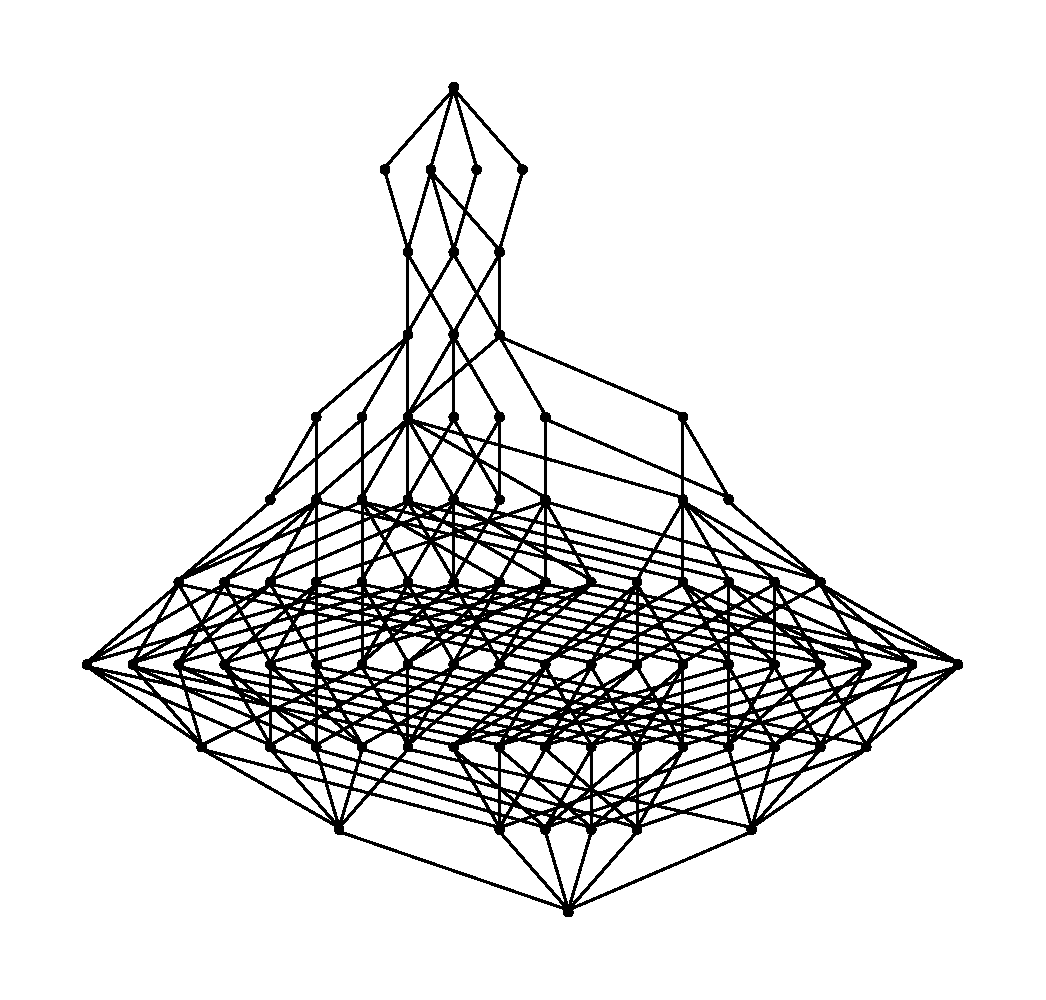
\includegraphics[width=\textwidth]{pics/ch-lattice/gossip3.pdf}
  \texttt{gap> Splash(DotString(LatticeOfCongruences(GossipMonoid(3))));}
  \caption[Congruence lattice of the Gossip monoid $G_3$]
  {Congruence lattice of the Gossip monoid $G_3$ \cite[\S2]{gossip}.  The
    semigroup contains $11$ elements, and the lattice contains $84$ congruences}
  \label{fig:g3-lattice}
\end{figure}

\begin{figure}[ht]
  \centering
  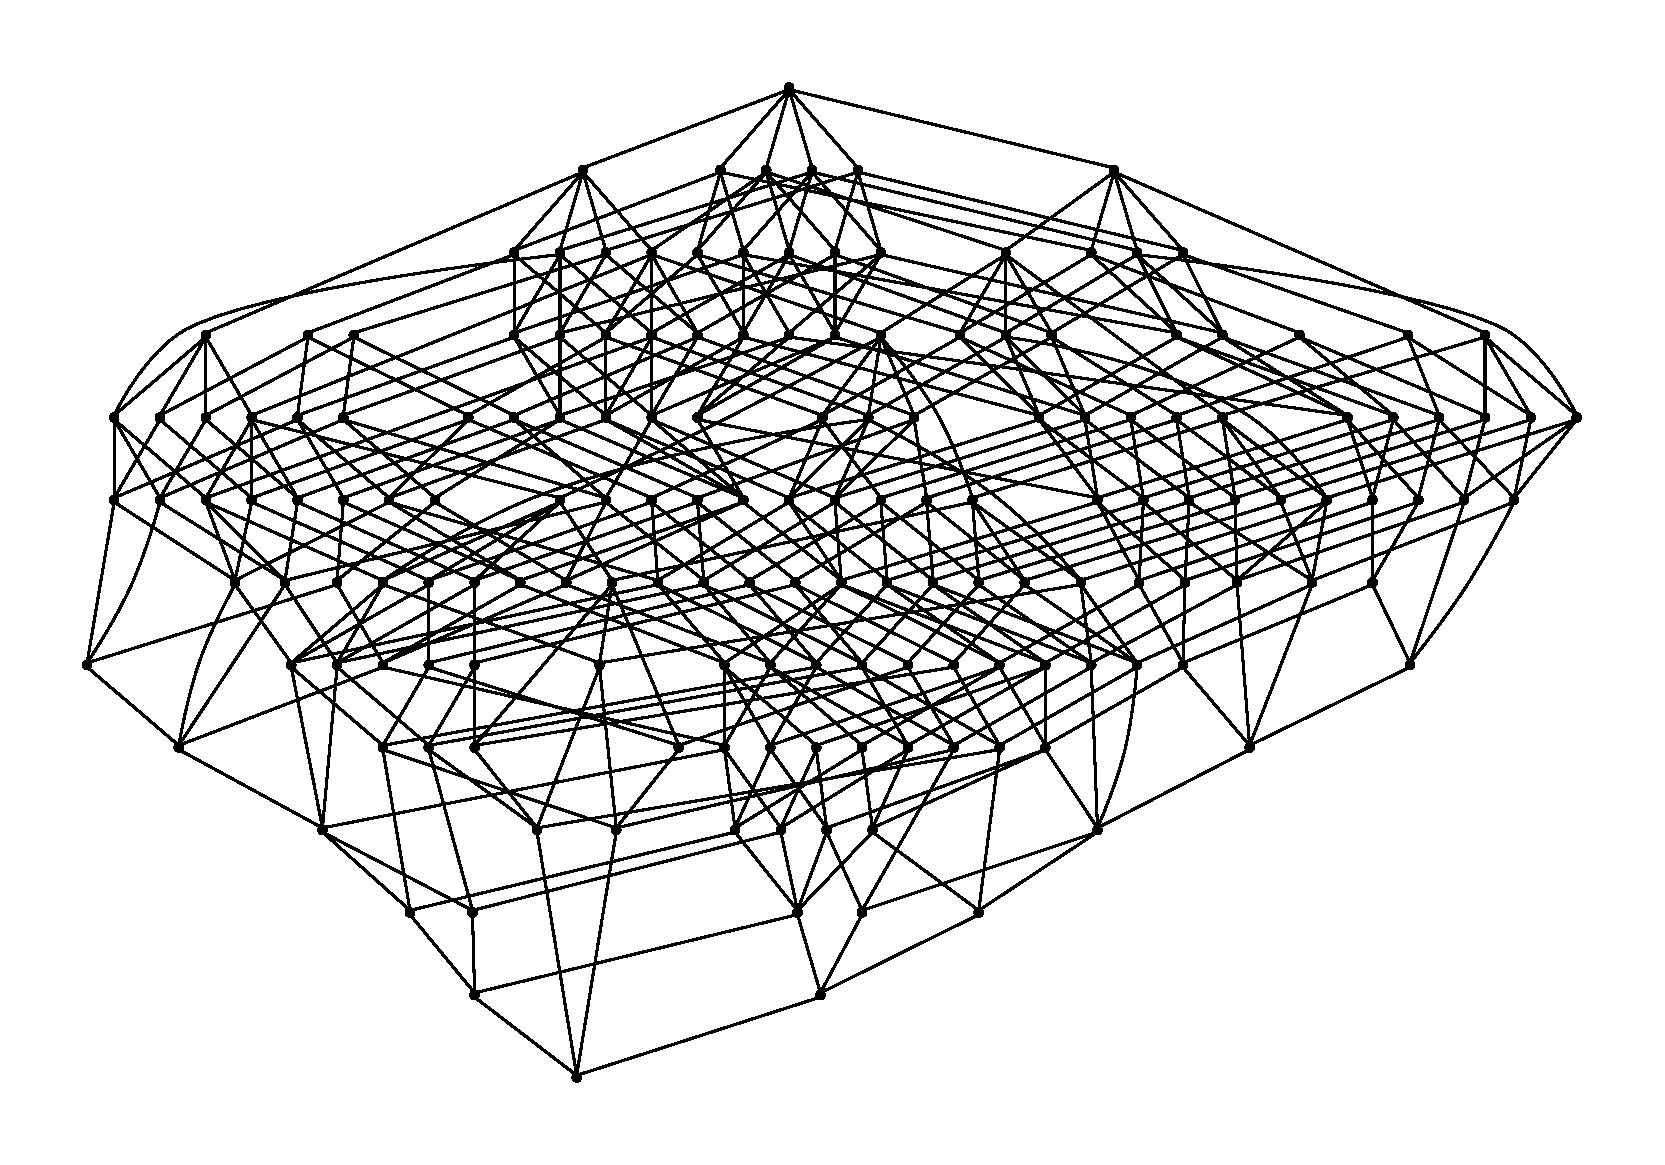
\includegraphics[width=\textwidth]{pics/ch-lattice/pbr1.pdf}
  \texttt{gap> Splash(DotString(LatticeOfCongruences(FullPBRMonoid(1))));}
  \caption[Congruence lattice of the full PBR monoid $\PBR_1$]
  {Congruence lattice of the full PBR monoid $\PBR_1$
    \cite[\S2.1]{diagram_semigroups}.  The semigroup contains $16$ elements, and
    the lattice contains $167$ congruences}
  \label{fig:pbr1-lattice}
\end{figure}

\begin{figure}[ht]
  \centering
  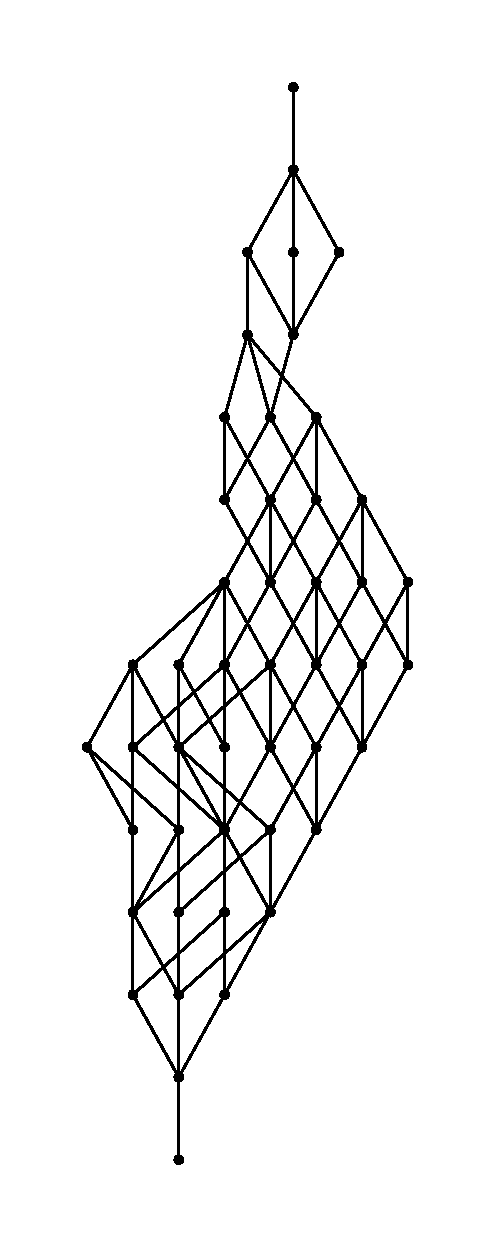
\includegraphics[height=0.8\textheight]{pics/ch-lattice/c2-wr-t3.pdf}
  \doublespacing
  \vspace{-1.5cm}
  \begin{align*}
    &\texttt{gap> C2 := Group((1, 2));;} \\
    &\texttt{gap> T3 := FullTransformationMonoid(3);;} \\
    &\texttt{gap> W := WreathProduct(C2, T3);;} \\
    &\texttt{gap> Splash(DotString(LatticeOfCongruences(W)));}
  \end{align*}
  \vspace{-1.0cm}
  \caption[Congruence lattice of the Wreath product $C_2 \wr \T_3$]
  {Congruence lattice of the Wreath product $C_2 \wr \T_3$
    \cite[\S10.1]{wreath}.  The semigroup contains $216$ elements, and the
    lattice contains $47$ congruences}
  \label{fig:c2-wr-t3-lattice}
\end{figure}

There are two main factors which determine how long
\texttt{LatticeOfCongruences} takes to compute the lattice: the size of the
semigroup $S$, and the number of congruences in the lattice $\Gamma$ itself.
Informal analysis shows that these two values do not necessarily go hand in
hand.  For instance, the monoids considered later in Section
\ref{sec:other-monoids-results} show a variety of numbers of congruences which
do not always correlate with the sizes of the semigroups.  Even Figures
\ref{fig:pbr1-lattice} and \ref{fig:c2-wr-t3-lattice} demonstrate between them
that an increase in semigroup size need not indicate an increase in number of
congruences.

In one test on an Intel Core i7-4770S CPU running at $3.10$GHz with 16GB of
memory, calculating the lattice of congruences of the wreath product
$C_2 \wr \T_3$ (Figure \ref{fig:c2-wr-t3-lattice}) took $3140$ ms, of which
almost all the time ($3019$ ms) was consumed by \textsc{PrincCongPoset}.  This
is because the semigroup is relatively large ($216$ elements), and therefore
iterating through all relevant pairs in $S \times S$ takes a long time; whereas
the number of congruences is relatively small (only $47$) meaning that the
taking of joins does not take long.  A contrasting example is the full PBR
monoid $\PBR_1$ (Figure \ref{fig:pbr1-lattice}): this took $5445$ ms in total,
of which almost all ($5422$ ms) was spent in \textsc{JoinClosure}.  This is
because the semigroup is relatively small (only $16$ elements), so iterating
through $S \times S$ is quick; but it has many congruences ($167$) meaning that
it takes a long time to compute all the joins.

Since it is unknown in advance how many congruences a semigroup has, it is
difficult to predict the feasibility of computing the lattice of a given
semigroup, even if its size is known.  Certainly all $853,303$ semigroups of
size up to $7$ have had their congruence lattices computed with the aid of the
\smallsemi{} library \cite{smallsemi}, and tests on randomly generated
transformation semigroups can usually calculate the lattice of a semigroup of
size up to 400 in less than a minute (on the previously mentioned computer).
However, we can choose very small examples in which \textsc{JoinClosure} runs
for an unreasonable amount of time.  Take, for example, the zero semigroup
$\Z_{10}$, with only $10$ elements.  Calculating all its congruences using the
method above does not complete within an hour, though computing the principal
congruences takes only $16$ milliseconds.  This is because $\Z_{10}$ has a large
number of congruences, given by the Bell number $B_{10} = 115975$, as will be
shown in Theorem \ref{thm:congruence-full}.  An alternative method would work
better here, since that theorem shows us that any equivalence on $\Z_{10}$ is a
congruence.

In both parts of the algorithm, most of the work consists of comparing
congruences to each other.  These comparisons can be done relatively quickly by
the efficient C++ code in \libsemigroups{} for generating pairs (see
Chapter \ref{chap:pairs}), but minimising the number of comparisons that need to
be made is nevertheless helpful for the algorithm's overall runtime.  Hence it
would be desirable, as future work, to improve the \textsc{PrincCongPoset}
algorithm somehow to avoid unnecessary comparisons, as well as to implement the
Froidure--Pin algorithm for \textsc{JoinClosure} in the \Semigroups{} package.

Since the algorithm described above was implemented in the \Semigroups{} package
\cite{semigroups}, it has been possible to compute the congruence lattice of
many semigroups.  Part \ref{part:results} of this thesis examines
the congruence lattices of a variety of semigroups, and attempts to explain
their structure.  Many of these lattices were originally computed using
\textsc{PrincCongPoset} and \textsc{JoinClosure}.  After examining these
lattices, it was possible in some cases to classify the congruences of entire
infinite families of semigroups, with proofs that were independent of any
computer code (see, for example, Theorems \ref{thm:mn-congs} and
\ref{thm:dkstar-congs}).  In others it was possible at least to produce
conjectures about families of semigroups, and to prove them for small cases (see
Conjectures \ref{conj:not-cong-full} and \ref{conj:cong-nearfull-7}).

\chapter{Converting between representations}
\label{chap:converting}

A congruence is a binary relation, and therefore is formally described as a set
of pairs -- a subset of $S \times S$.  In both computational and mathematical
settings, it is worth thinking about how a congruence could be stored.

One approach to storing a congruence $\rho$ on a semigroup $S$ is simply to
store every one of its pairs.  In principle, it is possible to store
$\rho$ in this way if and only if $S$ is finite.  However, this could well use a
lot of storage -- even the trivial congruence would use $O(|S|)$ space, and in
general a congruence could even use $O(|S|^2)$ space.

% TODO? quantify that we need very few pairs
In Chapter \ref{chap:pairs} we looked in detail at how a congruence can be
represented by a set of generating pairs.  As we found there, a congruence can
be described by a subset $\R \subseteq \rho$, which in many cases can be
very small.  This is one very generic way of representing congruences, in two
senses: firstly that it can be used for any finite semigroup; and secondly that
it can be used for left and right congruences.

However, there are other ways to view congruences in certain circumstances: some
semigroups have properties such as being an inverse semigroup or being a group,
which allow additional things to be said about their congruences; and some
specific congruences have special properties, such as being Rees, which allows
them to be represented in a certain way.  In this chapter, we will describe some
important ways of representing congruences, and then consider ways of converting
one to another.  Section numbers for the different representations and the ways
they can be converted to one another are summarised in Table
\ref{tab:converting}.

\begin{table}[ht]
  \centering
  \renewcommand{\arraystretch}{1.3}
  \begin{tabular}{ r | r | c | c | c | c | c |}
    \multicolumn{7}{c}{\qquad\qquad\qquad\qquad\qquad\qquad\qquad\qquad\qquad \ldots to \ldots} \\
    \cline{2-7}
    \multirow{7}{*}{\rotatebox[origin=c]{90}{From\ldots}} &  & GP & NS & LT & KT & RC \\
    \cline{2-7}
    & Generating pairs ~\ref{sec:converting-pairs} & \cellcolor{gray} & \ref{sec:trivial-conversions} & \ref{sec:pairs-to-linked-triple} & \ref{sec:pairs-to-kertr} & \textcolor{gray}{\ref{sec:pairs-to-rees}} \\
    \cline{2-7}
    & Normal subgroup (groups) ~\ref{sec:normal-subgroups} & \ref{sec:trivial-conversions} & \cellcolor{gray} & \ref{sec:normal-subgroup-to-linked-triple} & \ref{sec:trivial-conversions} & \ref{sec:trivial-conversions}\\
    \cline{2-7}
    & Linked triple ((0-)simple) ~\ref{sec:linked-triples} & \ref{sec:linked-triple-to-pairs} & \ref{sec:normal-subgroup-to-linked-triple} & \cellcolor{gray} & \ref{sec:trivial-conversions} & \ref{sec:trivial-conversions} \\
    \cline{2-7}
    & Kernel--trace (inverse) ~\ref{sec:kertr} & \textcolor{gray}{\ref{sec:kertr-to-pairs}} & \ref{sec:trivial-conversions} & \ref{sec:trivial-conversions} & \cellcolor{gray} & \ref{sec:rees-to-kertr} \\
    \cline{2-7}
    & Rees congruence ~\ref{sec:converting-rees} & \ref{sec:rees-to-pairs} & \ref{sec:trivial-conversions} & \ref{sec:trivial-conversions} & \ref{sec:rees-to-kertr} & \cellcolor{gray}\\
    \cline{2-7}
  \end{tabular}
  \renewcommand{\arraystretch}{0.7}
  \caption[References to conversion algorithms]
  {Section references to algorithms for converting between different congruence
    representations.  Grey references represent open problems.}
  \label{tab:converting}
\end{table}

\section{Ways of representing a congruence}
\label{sec:ways-of-representing}

We will begin by describing several different ways of representing a congruence.
These representations all exist in some form in \GAP{} \cite{gap} or the \Semigroups{}
package \cite{semigroups}.

\subsection{Generating pairs}
\label{sec:converting-pairs}
% TODO? Can RZMSNormalization improve this at all?
Recall that a congruence $\rho$ on a semigroup $S$ can be stored using
a subset of the pairs in $\rho$.  If $\R$ is a subset of $S \times S$,
then we can say that $\R$ \textit{generates} a congruence.  The
congruence \textit{generated by} $\R$ is defined as the least congruence
on $S$ containing all the pairs in $\R$; equivalently, it is defined as
the intersection of all congruences on $S$ containing all the pairs in
$\R$.  It is denoted by $\R^\sharp$ (see Theorem
\ref{thm:rsharp}).  We have similarly defined the left congruence generated by
$\R$ (denoted by $\R^\triangleleft$) and the right congruence
generated by $\R$ (denoted by $\R^\triangleright$).
A full explanation of how generating pairs can be used to represent congruences
is given in Section \ref{sec:intro-gen-pairs}, and an approach for computing
properties of congruences using their generating pairs is given in Chapter
\ref{chap:pairs}.

Given a set of pairs $\R$, we may wish to produce the congruence
$\R^\sharp$ and represent it using one of the other methods described in
this chapter.  It is of course possible to calculate the set of all pairs in
$\R^\sharp$ and convert that to the other representation; however, in
order to find other representations with as little work as possible, it is
desirable to use the pairs in $\R$ directly, calculating as few extra
pairs as possible -- see, for example, Sections \ref{sec:pairs-to-linked-triple}
and \ref{sec:pairs-to-kertr}.  Conversely, if we wish to convert another
representation for a congruence $\rho$ to a set of generating pairs, it is
desirable to find as small a set of pairs as possible -- see, for example,
Sections \ref{sec:linked-triple-to-pairs} and \ref{sec:rees-to-pairs}.  When
converting between generating pairs and other representations, these will be the
goals.

\subsection{Groups: normal subgroups}
\label{sec:normal-subgroups}

In group theory, it is unusual to encounter discussion of congruences.  This is
because a group's congruences are closely related to another structure -- its
normal subgroups -- and any questions we could ask about a group's congruences are
easily described using normal subgroups instead.  Recall that a subgroup $N$ of
a group $G$ is \textit{normal} if and only if $g^{-1}ng \in N$ for all $g \in G$
and $n \in N$; recall also that a \textit{coset} of $N$ is the set $Ng$ or $gN$
for some $g \in G$, and that $Ng=gN$ if $N$ is normal.  The following theorem
shows how a group's normal subgroups are in bijective correspondence with its
congruences.

\begin{theorem}
  \label{thm:normal-subgroups}
  Let $G$ be a group.  If $\rho$ is a congruence on $G$, then the $\rho$-class
  containing the identity is a normal subgroup of $G$.

  Conversely, if $N$ is a normal subgroup of $G$, then its cosets are the
  classes of a congruence on $G$.

  \begin{proof}
    First, let $\rho$ be a congruence on $G$, and let $I$ be the $\rho$-class
    containing the identity $1$.  First we show that $I$ is a subgroup: if
    $a,b \in I$ then $ab ~\rho~ 11 = 1$, so $ab \in I$.
    Furthermore, we have $(a,1) \in \rho$, so
    $(aa^{-1}, 1a^{-1}) = (1, a^{-1}) \in \rho$, so $a^{-1} \in I$, and so
    $I$ is a subgroup.  To show $I$ is normal, let $g \in G$ and $i \in I$.
    Observe that $g^{-1}ig ~\rho~ g^{-1}1g = g^{-1}g = 1$, so $g^{-1}ig \in I$,
    as required.

    To show the converse, let $N$ be a normal subgroup of $G$, and let $\nu$ be
    the equivalence on $G$ whose classes are the cosets of $N$.  If
    $(x,y), (s,t) \in \nu$, then $Nx=Ny$ and $sN=tN$.  Hence
    $Nxs=Nys=ysN=ytN=Nyt$, so we have $(xs,yt) \in \nu$, meaning that $\nu$ is
    a congruence as required.
  \end{proof}
\end{theorem}

This theorem means that any information which can be taken from a congruence can
instead be taken from a normal subgroup, and so congruences on a group need
never be studied directly.  We even have the fortunate property that the
containment of normal subgroups follows the containment of the corresponding
congruences.

It is possible to calculate the normal subgroups of a finite group relatively
quickly, using a variety of well-known algorithms.  One method for finding the
normal subgroups of a finite group is given in \cite{hulpke_1998}; this is the
method used in the most general case by \GAP{} \cite{gap}, though more specific
methods are used for certain specific categories of group.  In the case of an
infinite group, it may be impossible to find all normal subgroups -- indeed, this
problem is undecidable in general \cite[Theorem 3.17]{miller_1992} -- but the
\textsc{LowIndexSubgroups} algorithm \cite[\S 5.4]{cgt} may be used to find all
normal subgroups up to a given index, given a small modification to exclude
subgroups which are not normal \cite[\S 5.5]{cgt}.

The other structures discussed in this section represent congruences on other
categories of semigroup in a similar way.

\subsection{Completely (0-)simple semigroups: linked triples}
\label{sec:linked-triples}

There is a special way of describing a congruence on a completely simple or
completely 0-simple semigroup: using a linked triple.  We will start by
explaining the terms \textit{completely simple} and \textit{completely
  0-simple}, then we will define a semigroup's linked triples and explain how
they are related to its congruences.

\begin{definition}
  \label{def:zerosimple}
  \index{simple!semigroup}
  \index{0-simple}
  A semigroup $S$ is:
  \begin{itemize}
  \item \textbf{simple} if its only ideal is $S$;
  \item \textbf{0-simple} if it has a zero, and its only ideals are $S$ and
    $\{0\}$.
  \end{itemize}
\end{definition}

Simple and 0-simple semigroups are closely related.  Note that if $S$ is a
simple semigroup, then $S^0$, the semigroup created by appending a zero element
to $S$, is 0-simple.
Next, we consider a slightly stronger condition, after a preliminary definition
relating to idempotents.

\begin{definition}
  \label{def:primitive}
  \index{primitive idempotent}
  An idempotent $p \in S$ is \textbf{primitive} if it is non-zero and there is
  no other non-zero idempotent $i \in S$ such that $ip = pi = i$.
\end{definition}

\begin{definition}
  \label{def:completelyzerosimple}
  \index{completely!simple}
  \index{completely!0-simple}
  A semigroup is:
  \begin{itemize}
  \item \textbf{completely simple} if it is simple and contains a primitive
    idempotent;
  \item \textbf{completely 0-simple} if it is 0-simple and contains a primitive
    idempotent.
  \end{itemize}
\end{definition}

Definitions \ref{def:zerosimple} and \ref{def:completelyzerosimple} are
equivalent for finite semigroups -- that is to say, a finite semigroup is
completely simple if and only if it is simple, and it is completely 0-simple if
and only if it is 0-simple.  Some of the conversions described in this chapter
will be applicable only to finite semigroups, and in those circumstances we will
refer to \textit{finite simple} or \textit{finite 0-simple} semigroups, knowing
that these are completely simple or completely 0-simple, respectively.
Note that a finite semigroup is simple if and only if it is $\JJ$-trivial.

Completely simple and completely 0-simple semigroups have a strong and useful
isomorphism property, which allows us to say a great deal about their structure
and, in particular, their congruences.  We will consider first the more
complicated case, that of completely 0-simple semigroups, and then at the end of
this section we will explain how this theory can be adapted for the much less
complicated case, that of completely simple semigroups.

\begin{definition}[{\cite[\S 3.2]{howie}}]
  \label{def:rzms}
  \index{Rees 0-matrix semigroup}
  A \textbf{Rees 0-matrix semigroup} $\mathcal{M}^0[T;I,\Lambda;P]$ is the set
  $$(I \times T \times \Lambda) \cup \{0\}$$
  with multiplication given by
  $$(i,a,\lambda) \cdot (j,b,\mu) = \left\{
    \begin{array}{l l}
      (i,ap_{\lambda j}b, \mu) & \text{if~} p_{\lambda j} \neq 0, \\
      0 & \text{otherwise,}
    \end{array}
  \right.$$
  where
  \begin{itemize}
  \item $T$ is a semigroup,
  \item $I$ and $\Lambda$ are index sets,
  \item $P$ is a $|\Lambda| \times |I|$ matrix with entries $(p_{\lambda
      i})_{\lambda \in \Lambda, i \in I}$
    taken from $T^0$,
  \item $0x=x0=0$ for all $x \in \mathcal{M}^0[T;I,\Lambda;P]$.
  \end{itemize}
\end{definition}

We will require a certain property of the matrix $P$, which we should define
first: we call a matrix \textbf{regular} \index{regular!matrix} if it contains
at least one non-zero entry in each row and each column.

The following theorem shows how we can use Rees 0-matrix semigroups to classify
completely 0-simple semigroups.

\begin{theorem}[Rees]
  \label{thm:rees}
  Every completely 0-simple semigroup is isomorphic to a Rees 0-matrix semigroup
  $\mathcal{M}^0[G;I,\Lambda;P]$, where $G$ is a group and $P$ is regular.
  Conversely, every such Rees 0-matrix semigroup is completely 0-simple.
  \begin{proof}
    Theorem 3.2.3 in \cite{howie}.
  \end{proof}
\end{theorem}

Now we can replace any completely 0-simple semigroup with its isomorphic Rees
0-matrix semigroup when we wish to perform any isomorphism-invariant
calculations -- hence we can restrict our further investigations just to this
type of semigroup.  Note that if $\mathcal{M}^0[G;I,\Lambda;P]$ is finite, then
$G$, $I$, $\Lambda$ and $P$ are all finite.

Next we consider the congruences of a finite 0-simple semigroup.

\begin{definition}
  \label{def:linked-triple}
  \index{linked triple}
% \nomenclature[N,S,T]{$(N,\sS,\tT)$}{Linked triple}
  \nomenclature[S]{$\sS$}{Relation on column set $I$}
  \nomenclature[T]{$\tT$}{Relation on row set $\Lambda$}
  Let $S$ be a finite Rees 0-matrix semigroup $\mathcal{M}^0[G;I,\Lambda;P]$
  over the group $G$ with regular matrix $P$.  A \textbf{linked triple} on $S$
  is a triple $$(N,\mathcal{S},\mathcal{T})$$ consisting of a normal subgroup
  $N \trianglelefteq G$, an equivalence relation $\mathcal{S}$ on $I$ and an
  equivalence relation $\mathcal{T}$ on $\Lambda$, such that the following are
  satisfied:
  \begin{enumerate}[\rm(1)]
  \item $\mathcal{S} \subseteq \varepsilon_I$, where $\varepsilon_I =
    \left\{(i,j) \in I \times I\, \middle|\, \forall \lambda \in \Lambda:
      p_{\lambda i}=0 \iff p_{\lambda j}=0 \right\}$,
  \item $\mathcal{T} \subseteq \varepsilon_\Lambda$, where $\varepsilon_\Lambda
    = \left\{(\lambda,\mu) \in \Lambda \times \Lambda\, \middle|\, \forall i \in
      I: p_{\lambda i}=0 \iff p_{\mu i}=0 \right\}$,
  \item For all $i,j \in I$ and $\lambda, \mu \in \Lambda$ such that
    $p_{\lambda i}, p_{\lambda j}, p_{\mu i}, p_{\mu j} \neq 0$ and either
    $(i,j) \in \mathcal{S}$ or $(\lambda,\mu) \in \mathcal{T}$, we have
    $q_{\lambda \mu i j} \in N$, where
    $$q_{\lambda \mu i j} = p_{\lambda i} p_{\mu i}^{-1} p_{\mu j} p_{\lambda
      j}^{-1}.$$
  \end{enumerate}
  \cite[\S 3.5]{howie}
\end{definition}

We can associate the linked triples of a finite 0-simple semigroup with its
non-universal congruences, as follows.

\begin{theorem}
  \label{thm:linked-triple}
  Let $S$ be a Rees 0-matrix semigroup defined with a group and a regular
  matrix.  There exists a bijection $\Gamma$ between the non-universal
  congruences on $S$ and the linked triples on $S$.
  \begin{proof}
    Theorem 3.5.8 in \cite{howie}
  \end{proof}
\end{theorem}

This theorem shows us an alternative way to look at congruences on completely
0-simple semigroups, just as normal subgroups show us an alternative way to look
at congruences on groups.  However, in order to use this at all in a
computational setting, we must have a concrete function $\Gamma$ which we can
use to convert a congruence to a linked triple and back again, rather than just
the knowledge that such a function exists -- indeed, describing such a function
is the purpose of this section.  We define the function $\Gamma$ as follows.

\begin{definition}[{\cite[\S 3.5]{howie}}]
  \label{def:linked-triple-function}
  \index{linked triple!function}
  Let $S$ be a Rees 0-matrix semigroup $\mathcal{M}^0[G;I,\Lambda;P]$ over a
  group $G$ and a regular matrix $P$, and let $\rho$ be a non-universal
  congruence on $S$.
  The \textbf{linked triple function} of $S$ is the function
  $$\Gamma: \rho \mapsto (N_\rho, \mathcal{S}_\rho, \mathcal{T}_\rho),$$
  which maps any non-universal congruence onto a triple whose entries are
  defined as follows.

  The relation $\mathcal{S}_\rho \subseteq I \times I$ is defined by the rule that
  $(i,j) \in \mathcal{S}_\rho$ if and only if $(i,j) \in \varepsilon_I$ and
  $$(i, p_{\lambda i}^{-1}, \lambda) ~\rho~ (j, p_{\lambda j}^{-1}, \lambda)$$
  for all $\lambda \in \Lambda$ such that $p_{\lambda i} \neq 0$ (and hence
  $p_{\lambda j} \neq 0$).  Similarly, the relation
  $\mathcal{T}_\rho \subseteq \Lambda \times \Lambda$ is defined by the rule that
  $(\lambda,\mu) \in \mathcal{T}_\rho$ if and only if
  $(\lambda,\mu) \in \varepsilon_\Lambda$ and
  $$(i, p_{\lambda i}^{-1}, \lambda) ~\rho~ (i, p_{\mu i}^{-1}, \mu)$$
  for all $i \in I$ such that $p_{\lambda i} \neq 0$ (and hence
  $p_{\mu i} \neq 0$).  Finally, we define the normal subgroup
  $N_\rho \trianglelefteq G$ as follows.  First, fix some $\xi \in \Lambda$, a
  row of the matrix $P$.  Since $P$ is regular, row $\xi$ must contain a
  non-zero entry -- fix some $k \in I$ such that $p_{\xi k} \neq 0$.  Now we can
  define
  $$N_\rho = \{a \in G ~|~ (k, a, \xi) ~\rho~ (k, 1_G, \xi)\},$$
  where $1_G$ is the identity in the group $G$.
  The inverse of $\Gamma$ is then such that
  $(N, \mathcal{S}, \mathcal{T})\Gamma^{-1}$ is equal to
  $$\Big\{
  \big((i, a, \lambda), (j, b, \mu)\big) ~\Big|~
  (p_{\xi i} a p_{\lambda x}) (p_{\xi j} b p_{\mu x})^{-1} \in N,
  (i,j) \in \mathcal{S},
  (\lambda,\mu) \in \mathcal{T}
  \Big\},$$
  where $\xi \in \Lambda$ and $x \in I$ can be any elements such that
  $p_{\xi i}$ and $p_{\lambda x}$ are both non-zero.
\end{definition}

Note that the definition of $N_\rho$ does not depend on the choice of $\xi$ and
$k$.  Independence from the choice of $\xi$ is established by the following
lemma, and independence from the choice of $k$ follows by a similar argument.

\begin{lemma}
  Let $\xi_1, \xi_2 \in \Lambda$ and $k \in I$ such that $p_{\xi_1k}^{} \neq 0$
  and $p_{\xi_2 k}^{} \neq 0$.  Then
  $$(k, a, \xi_1) ~\rho~ (k, 1_G, \xi_1)
  \quad \text{if and only if} \quad
  (k, a, \xi_2) ~\rho~ (k, 1_G, \xi_2)$$
  for all $a \in G$.
  \begin{proof}
    Assume that $(k, a, \xi_1) ~\rho~ (k, 1_G, \xi_1)$.  We can right-multiply
    both sides by $(k, p_{\xi_1k}^{-1}, \xi_2)$ to give
    $$(k, a, \xi_1)(k, p_{\xi_1k}^{-1}, \xi_2)
    ~\rho~ (k, 1_G, \xi_1)(k, p_{\xi_1k}^{-1}, \xi_2),$$
    which simplifies to
    $$(k, a p_{\xi_1k}^{} p_{\xi_1k}^{-1}, \xi_2)
    ~\rho~ (k, 1_G p_{\xi_1k}^{} p_{\xi_1k}^{-1}, \xi_2),$$
    and then to
    $(k, a, \xi_2) ~\rho~ (k, 1_G, \xi_2)$,
    as required.
    The converse argument is identical, swapping $\xi_1$ for $\xi_2$.
  \end{proof}
\end{lemma}

\index{Rees matrix semigroup}
Our discussion so far has focused on 0-simple semigroups, but very similar
structures exist for completely \textit{simple} semigroups.  They are isomorphic
to \textbf{Rees matrix semigroups}, and linked triples can be defined on them in
almost exactly the same way, except for the removal of complications related to
the zero element.  A Rees matrix semigroup follows Definition \ref{def:rzms} but
with the removal of the zero element, and linked triples follow Definition
\ref{def:linked-triple}, where the restrictions related to placements of $0$ in
$P$ are irrelevant.  It should also be noted that even the universal congruence
has a linked triple in this
case -- $(G, I \times I, \Lambda \times \Lambda)$ -- so the domain of $\Gamma$ is
not only the non-universal congruences, but all congruences on $S$.

\subsection{Inverse semigroups: kernel--trace pairs}
\label{sec:kertr}
% TODO? Wilf's book about semilattice congruences: Symmetric Inverse Semigroups

An inverse semigroup also has a structure which can be used in place of its
congruences: its \textit{kernel--trace pairs} (sometimes confusingly known as
``congruence pairs'').  In \cite[Chapter 5]{mtorpey_msc} the author focused on a
computational use of kernel--trace pairs to solve problems about congruences.
They can certainly be used effectively to carry out calculations, in a similar
way to linked triples.

The basic theory about kernel--trace pairs is presented here, for reference.  In
all these definitions, $S$ is an inverse semigroup, $E$ is the set of
idempotents in $S$, and and $\rho$ is a congruence on $S$.  Recall that $E$ is
an inverse subsemigroup of $S$.  This is standard background theory, which is
adapted from \cite[\S 5.3]{howie}.

\begin{definition}
  \label{def:kernel-cong}
  \index{kernel!of a congruence}
  The \textbf{kernel} of $\rho$ is $\bigcup_{e \in E} [e]_\rho$, the union of
  all the $\rho$-classes of $S$ which contain idempotents.  It is denoted by
  $\ker\rho$.
\end{definition}

\begin{definition}
  \label{def:trace}
  \index{trace}
  The \textbf{trace} of $\rho$ is $\rho \cap (E \times E)$, the restriction of
  $\rho$ to the idempotents of $S$.  It is denoted by $\tr\rho$.
\end{definition}

We will shortly see that a congruence on $S$ is completely defined by its kernel
and trace.  First we will approach kernel--trace pairs from an abstract route
which will help us to classify the congruences on $S$ completely.  We start with
two different definitions of the word ``normal'', one for subsemigroups and one
for congruences.

\begin{definition}
  \label{def:kernel-normal}
  \index{normal!subsemigroup}
  A subsemigroup $K$ of $S$ is called \textbf{normal} if it is
  \textit{full} (contains all the idempotents of $S$) and
  \textit{self-conjugate} ($a^{-1}xa \in K$ for all $x \in K, a \in S$).
\end{definition}

\begin{definition}
  \label{def:trace-normal}
  \index{normal!congruence}
  A congruence $\tau$ on $E$ is \textbf{normal} in $S$ if
  $$(a^{-1}ea,a^{-1}fa) \in \tau$$
  for every pair $(e,f) \in \tau$ and every element $a \in S$.
\end{definition}

Now we can define a \textit{kernel--trace pair}, an abstract structure which
relates very closely to a congruence.

\begin{definition}
  \label{def:kernel-trace-pair}
  \index{kernel--trace pair!for an inverse semigroup}
  A \textbf{kernel--trace pair} on $S$ is a pair $(K,\tau)$ consisting of a
  normal subsemigroup $K$ of $S$ and a normal congruence $\tau$ on $E$, such
  that
  \begin{enumerate}[\rm(1)]
  \item If $ae \in K$ and $(e,a^{-1}a) \in \tau$, then $a \in K$
  \item If $a \in K$, then $(aa^{-1},a^{-1}a) \in \tau$
  \end{enumerate}
  for all elements $a \in S$ and $e \in E$.
\end{definition}

Now we state the result which identifies an abstract kernel--trace pair with the
kernel and trace of a congruence, and allows us to calculate information about
$\rho$ by using $\ker \rho$ and $\tr \rho$ directly.

\begin{theorem}
  \label{thm:kernel-trace-pair}
  % Let $\rho$ be a congruence on an inverse semigroup $S$ with idempotent
  % semigroup $E$.  $(\ker\rho, \tr\rho)$ is a kernel--trace pair.

  % Conversely, every kernel--trace pair $(K,\tau)$ on $S$ defines a congruence
  % $$\rho_{(K,\tau)} = \{(x,y) \in S \times S ~|~ (x^{-1}x, y^{-1}y) \in \tau,
  % xy^{-1} \in K\}$$
  % whose kernel is equal to $K$ and whose trace is equal to $\tau$.  Finally,
  % $\rho_{(\ker\rho,\tr\rho)} = \rho$.
  Let $S$ be an inverse semigroup.  There exists a bijection $\Psi$ from the
  congruences on $S$ to the kernel--trace pairs on $S$, defined by
  $$\Psi: \rho \mapsto (\ker\rho, \tr\rho),$$
  and its inverse satisfies
  $$\Psi^{-1} : (K,\tau) \mapsto
  \{(x,y) \in S \times S ~|~ xy^{-1} \in K, (x^{-1}x, y^{-1}y) \in \tau\}.$$
  \begin{proof}
    Theorem 5.3.3 in \cite{howie}.
  \end{proof}
\end{theorem}

This theorem tells us everything we need to know about kernel--trace pairs and
their relationship to congruences on an inverse semigroup.  Once we have the
kernel--trace pair of a congruence, we can solve any problem we wish to using the
kernel and trace alone, and computational problems such as determining whether a
given pair $(x,y)$ lies in the congruence are much faster than using
generating pairs directly \cite[\S 6.1.3]{mtorpey_msc}.  However, we may find
that if a congruence is specified initially using generating pairs, it may be
costly to find its kernel--trace pair in the first place; Section
\ref{sec:pairs-to-kertr} presents a relatively fast method for finding a kernel--trace pair.

\subsection{Rees congruences}
\label{sec:converting-rees}
Recall that a \textit{Rees congruence} is a congruence on a semigroup $S$ with a
distinguished congruence class $I$ which is a two-sided ideal of $S$, and in
which every other congruence class is a singleton.  We may write this congruence
as $\rho_I$, and we may write its quotient $S/\rho_I$ as $S/I$.  Hence, a pair
$(x,y)$ lies in $\rho_I$ if and only if $x=y$ or $x$ and $y$ both lie in $I$.

Some or all of a semigroup's congruences may be Rees: in particular, since $S$
is an ideal of $S$, the universal congruence $S \times S$ is a Rees congruence
which could be written as $\rho_S$.  If $S$ has a zero $0$, then $\{0\}$ is an
ideal and so the trivial congruence $\Delta_S$ is a Rees congruence which could
be written as $\rho_{\{0\}}$.

As an example, the monoid of all order-preserving transformations $\OO_n$ has
only Rees congruences, apart from the trivial congruence $\Delta_{\OO_n}$, which
is not Rees, since $\OO_n$ does not contain a zero \cite{lavers_1999}.
Some examples of semigroups whose congruences are all Rees can be found in
\cite[\S 5]{garcia_1991}.

\section{Converting between representations}
\label{sec:converting}

In Section \ref{sec:ways-of-representing} we presented five different ways of
representing a congruence.  In this section, we present a survey of the
different ways in which they can be converted to each other.  Table
\ref{tab:converting} summarises the methods which exist, and the sections in
which they are described.

\subsection{Normal subgroups and linked triples}
\label{sec:normal-subgroup-to-linked-triple}
In this section we will consider how to convert between a normal subgroup (which
represents a congruence on a group) and a linked triple (which represents a
congruence on a simple semigroup).  This conversion is rather trivial, but is
presented as a good example of how different congruence representations can be
closely related.

Any group is a completely simple semigroup.  In fact, since any group $G$ has
precisely one $\HH$-class, it is isomorphic to the Rees matrix semigroup
$\mathcal{M}[G; I, \Lambda; P]$ where $|I|=|\Lambda|={1}$ and $P$ is the
$1 \times 1$ matrix $(1_G)$.  Let $\phi: G \to \mathcal{M}[G; I, \Lambda; P]$ be
the isomorphism defined by $(g)\phi = (1, g, 1)$.

As described in Theorem \ref{thm:normal-subgroups}, a congruence $\rho$ on a
group $G$ is associated with a normal subgroup $N \trianglelefteq G$, according
to the rule that $x ~\rho~ y$ if and only if $xy^{-1} \in N$.  Similarly, as
described in Definition \ref{def:linked-triple-function}, a congruence $\rho'$
on $\mathcal{M}[G; I, \Lambda; P]$ is associated with a linked triple
$(N', \mathcal{S}, \mathcal{T})$, according to the rule that
$(i, a, \lambda) ~\rho~ (j, b, \mu)$ if and only if $i ~\mathcal{S}~ j$,
$\lambda ~\mathcal{T}~ \mu$, and
$(p_{1 i} a p_{\lambda 1}) (p_{1 j} b p_{\mu 1})^{-1} \in N'$.
Since $|I|=|\Lambda|={1}$ and $P=(1_G)$, this last condition simplifies to
$ab^{-1} \in N'$.

Let $\rho'$ be the congruence on $\mathcal{M}[G; I, \Lambda; P]$ such that
$(x)\phi ~\rho~ (y)\phi$ (i.e.~$(1,x,1) \mathrel{\rho'} (1,y,1)$) if and only if
$x ~\rho~ y$.  The condition defining $\rho$, that $xy^{-1} \in N$, is
equivalent to the condition defined by the linked triple
$(N, \Delta_I, \Delta_\Lambda)$, since $I$ and $\Lambda$ are both trivial.
Hence any normal subgroup $N$ corresponds to the linked triple
$(N, \Delta_I, \Delta_\Lambda)$, making linked triples on groups very easy to
deal with.

\subsection{Generating pairs of a Rees congruence}
\label{sec:rees-to-pairs}
A natural question, given an ideal $I$, is how to find a set of generating pairs
for the Rees congruence $\rho_I$.  In this section we will limit our discussion
to finite semigroups.

\begin{theorem}
  Let $S$ be a finite semigroup, and let $I$ be an ideal of $S$.  If $X$ is an ideal
  generating set for $I$ (see Section \ref{sec:intro-ideals}) and $M$
  is the minimal ideal of $S$ (which may or may not be equal to $I$), then
  $$X \times M$$ is a set of generating pairs for the Rees congruence $\rho_I$.
  \begin{proof}
    Let $\rho$ be the congruence generated by $X \times M$.  First we show that
    $\rho \subseteq \rho_I$, and then that $\rho_I \subseteq \rho$.

    Let $(i,m) \in X \times M$.  We have $X \subseteq I$ since $X$ is a
    generating set for $I$, and $M \subseteq I$ since $M$ is contained in any
    ideal of $S$.  Hence $i$ and $m$ both lie in $I$, so they are in the same
    class of the Rees congruence: $(i,m) \in \rho_I$.  Hence $X \times M
    \subseteq \rho_I$, and so $\rho$ (the least congruence containing $X \times
    M$) must also be contained in $\rho_I$.  Hence $\rho \subseteq \rho_I$.

    Now let $(a,b) \in \rho_I$; we wish to show that $(a,b) \in \rho$.  If $a=b$
    then we certainly have $(a,b) \in \rho$.  Otherwise we must have $a,b \in
    I$.  Since $X$ \textit{generates} $I$, we have $I = S^1XS^1$.  Therefore we
    can write
    $$a = s_1x_1t_1, \quad b = s_2x_2t_2,$$
    for some $x_1,x_2 \in X$ and $s_1,s_2,t_1,t_2 \in S^1$.

    Now choose some $m \in M$.  By definition $(x_1,m), (x_2,m) \in \rho$ since
    $X \times M \subseteq \rho$, and
    by the compatibility properties of a congruence,
    $$(s_1x_1t_1,s_1mt_1), (s_2x_2t_2,s_2mt_2) \in \rho.$$

    Since $m \in M$, we must have $s_1mt_1,s_2mt_2 \in M$.  Let $x_0$ be an
    arbitrary element of $X$.
    We see $(x_0,s_1mt_1), (x_0,s_2mt_2) \in X \times M$, and so by transitivity
    $(s_1mt_1, s_2mt_2) \in \rho$.
    Hence
    $$a ~=~ s_1x_1t_1 ~\rho~ s_1mt_1 ~\rho~ s_2mt_2 ~\rho~ s_2x_2t_2 = b,$$
    and $(a,b) \in \rho$ as required.
  \end{proof}
\end{theorem}

\subsection{Linked triple from generating pairs}
\label{sec:pairs-to-linked-triple}

In \cite[\S 6.1]{mtorpey_pre_msc} it is observed that calculating information
about a congruence using its linked triple is much faster than using a set of
generating pairs.  However, it may well be that a congruence on a finite
simple or finite 0-simple semigroup is specified by generating pairs, and we do
not know its linked triple \textit{a priori}.  In this case, we will need to
calculate the congruence's linked triple before we can use it to calculate any
other information.  We could do this by enumerating all the elements of all the
classes of the congruence, and then simply looking up the relevant information
to find the linked triple.  However, this is very expensive, and once the
classes are enumerated there is likely no need for the linked triple, since all
information about the congruence has been calculated.

In \cite[\S 3.2]{mtorpey_msc}, the author presents an algorithm to calculate a
congruence's linked triple directly from a set of generating pairs, calculating
as few extra pairs as possible.  This algorithm performs quickly, representing a
big improvement on using a more naive algorithm to find the linked triple
\cite[\S 6.1.2]{mtorpey_msc}.  The algorithm is justified by the following
definition and theorem from \cite{mtorpey_msc}.

\begin{definition}[{\cite[Definition 3.10]{mtorpey_msc}}]
  \label{def:ri}
  Let $S = \mathcal{M}^0[G;I,\Lambda;P]$ be a finite Rees 0-matrix semigroup
  over a group $G$ with regular matrix $P$, and let $\R \subseteq S \times S$ be
  a relation on it.  We define the relations $\R|_I$ and $\R|_\Lambda$ by
  $$\R|_I = \big\{(i,j) \in I \times I ~\big|~
  (i,a,\lambda) ~\R~ (j,b,\mu)\big\},$$
  % ~\text{for some}~a,b \in G,~\lambda,\mu \in \Lambda\big\},$$
  $$\R|_\Lambda = \big\{(\lambda,\mu) \in \Lambda \times \Lambda ~\big|~
  (i,a,\lambda) ~\R~ (j,b,\mu)\big\}.$$
  % ~\text{for some}~a,b \in G,~i,j \in I\big\}.$$
\end{definition}

\begin{theorem}[{\cite[Theorem 3.11]{mtorpey_msc}}]
  \label{thm:pairs-to-linked-triple}
  Let $S = \mathcal{M}^0[G;I,\Lambda;P]$ be a finite 0-simple semigroup over a
  group $G$ with regular matrix $P$, with a relation $\R \subseteq S \times S$
  that generates a non-universal congruence $\R^\sharp$.  Let
  $\mathcal{S}_{\Rs} = (\R|_I)^e$, let
  $\mathcal{T}_{\Rs} = (\R|_\Lambda)^e$, and let $N_{\Rs}$ be
  the least normal subgroup of $G$ containing the set
  \begin{align*}
    \Big\{(p_{\xi i} a p_{\lambda x}) (p_{\xi j} b p_{\mu x})^{-1} ~\Big|~
    & i,j,x \in I,\ \lambda, \mu, \xi \in \Lambda,\ a,b \in G \\
    & \text{such that~} (i,a,\lambda) ~\R~ (j,b,\mu) \text{~and~}
      p_{\xi i}, p_{\lambda x} \neq 0\Big\} \\
    \cup~ \Big\{q_{\lambda \mu i j} ~\Big|~ &
           (i,j) \in \R|_I,~
           \lambda,\mu \in \Lambda ~\textnormal{such that}~
           p_{\lambda i}, p_{\mu i} \neq 0\Big\} \\
    \cup~ \Big\{q_{\lambda \mu i j} ~\Big|~ &
           (\lambda,\mu) \in \R|_\Lambda,~
           i,j \in I ~\textnormal{such that}~
           p_{\lambda i}, p_{\lambda j} \neq 0\Big\}. \\
  \end{align*}
  Then $(N_{\Rs}, \mathcal{S}_{\Rs}, \mathcal{T}_{\Rs})$
  is the linked triple corresponding to $\R^\sharp$.
\end{theorem}

This theorem is enough to show the correctness of our algorithm for converting a
set of generating pairs to a linked triple -- we present this algorithm here as
Algorithm \ref{alg:pairs-to-linked-triple}.  In reading the algorithm, it will
be helpful to refer to Definition \ref{def:linked-triple} for the relations
$\varepsilon_I$ and $\varepsilon_\Lambda$ and elements of the form
$q_{\lambda \mu i j}$.  The notation $\llangle N, x \rrangle$ describes the
least normal subgroup of $G$ containing $N \cup \{x\}$ (see Definition
\ref{def:normal-closure}); in particular, this is equal to $N$ if $x \in N$.
For a fuller description of the algorithm and how it is justified by Theorem
\ref{thm:pairs-to-linked-triple}, see \cite[\S 3.2]{mtorpey_msc}.

\begin{algorithm}
\caption{The \textsc{LinkedTripleFromPairs} algorithm}
\label{alg:pairs-to-linked-triple}
\index{LinkedTripleFromPairs@\textsc{LinkedTripleFromPairs}}
\begin{algorithmic}[1]
    \Require $\mathcal{M}^0[G;I,\Lambda;P]$ a finite Rees 0-matrix semigroup
    \Require $G$ a group, $P$ a regular matrix
    \Procedure{LinkedTripleFromPairs}{$\R$}
      \State $N := \{1_G\}$
      \State $\mathcal{S} := \Delta_I$
      \State $\mathcal{T} := \Delta_\Lambda$
      \For{$(x,y) \in \R$}
        \If{$x=y$}
          \State \Continue
        \ElsIf{$x=0 \Or y=0$}
          \State \Return Universal Congruence (no linked triple)
        \EndIf
        \State Let $x=(i,a,\lambda)$
        \State Let $y=(j,b,\mu)$
        \If{$(i,j) \notin \varepsilon_I \Or
          (\lambda,\mu) \notin \varepsilon_\Lambda$}
          \State \Return Universal Congruence (no linked triple)
        \EndIf

%        \State
        \LComment{Combine row and column classes}
        \State $\sS \gets \left(\sS \cup (i,j)\right)^e$
        \State $\tT \gets \left(\tT \cup (\lambda, \mu)\right)^e$

%        \State
        \LComment{Add generators for normal subgroup}
        \State Choose $\nu \in \Lambda$ such that $p_{\nu i} \neq 0$
        \State Choose $k \in I$ such that $p_{\lambda k} \neq 0$
        \State $N \gets \llangle N, (p_{\nu i}ap_{\lambda k})(p_{\nu j}bp_{\mu k})^{-1} \rrangle$

%        \State
        \For{$\xi \in \Lambda \setminus \{\nu\}$ such that $p_{\xi i} \neq 0$}
          \State $N \gets \llangle N, q_{\nu \xi i j} \rrangle$
        \EndFor
        \For{$x \in I \setminus \{k\}$ such that $p_{\lambda x} \neq 0$}
          \State $N \gets \llangle N, q_{\lambda \mu k x} \rrangle$
        \EndFor
      \EndFor
      \State \Return $(N,\mathcal{S},\mathcal{T})$
    \EndProcedure
\end{algorithmic}
\end{algorithm}

We can see the algorithm working in the following example.

\begin{example}
  \label{ex:pairs-to-linked-triple-4x2}
  Let $S = \mathcal{M}^0[\mathcal{D}_4; \{1,2,3,4\}, \{1,2\}; P]$ be a Rees
  0-matrix semigroup, where $\mathcal{D}_4$ is the permutation group
  $\langle (1~2~3~4), (2~4) \rangle$, isomorphic to the dihedral group on $4$
  points, and $P$ is the $2 \times 4$ matrix
  $$
  \begin{pmatrix}
    0 & (1~2)(3~4) & 0 & (1~4~3~2) \\
    (2~4) & (1~4)(2~3) & (2~4) & 0
  \end{pmatrix}.
  $$
  Let $\rho$ be the congruence generated by the single pair
  $\left(\left(1, (), 1\right), \left(3, (1~2~3~4), 1\right)\right)$.  We can
  use \textsc{LinkedTripleFromPairs} to find the linked triple corresponding to
  $\rho$, or to determine that $\rho$ is universal.

  We set our triple to $(\{()\}, \Delta_4, \Delta_2)$ to start with, where
  $\Delta_n$ is the diagonal relation on $\{1, \ldots, n\}$.  Then we consider
  the single pair in the generating set: $x = \left(1, (), 1\right)$ and
  $y = \left(3, (1~2~3~4), 1\right)$.  We do not have $x=y$, $x=0$ or $y=0$, so
  we go on to consider the two elements componentwise.  The pair $(i,j) = (1,3)$
  lies in $\varepsilon_I$ since columns $1$ and $3$ contain zeroes in the same
  positions, and $(\lambda,\mu) = (1,1)$ certainly lies in $\varepsilon_\Lambda$
  since it is a reflexive pair; hence we do not have to return the universal
  congruence.  We modify $\sS$ by joining the classes of $1$ and $3$ together;
  we do not have to modify $\tT$, since $(1,1)$ is already in $\tT$.  Finally we
  have to add generators to $N$: we can set both $\nu$ and $k$ to $2$, and then
  we add to $N$ the element
  \begin{align*}
    (p_{\nu i}ap_{\lambda k})(p_{\nu j}bp_{\mu k})^{-1}
    &= \left(p_{2 1}()p_{1 2}\right)\left(p_{2 3}(1~2~3~4)p_{1 2}\right)^{-1} \\
    &= \left((2~4)()(1~2)(3~4)\right)\left((2~4)(1~2~3~4)(1~2)(3~4)\right)^{-1}\\
    &= (1~2~3~4),
  \end{align*}
  and take the normal closure.  Finally we have to add any appropriate $q$
  values.  There is no value of $\xi$ which meets the stated requirements, but
  there is one appropriate value for $x$: $x = 4$.  Hence we have to add the
  element
  $q_{\lambda \mu k x}
  = q_{1 1 2 4}
  = p_{1 2} p_{1 2}^{-1} p_{1 4} p_{1 4}^{-1}
  = ()$.
  Since the identity already lies in $N$, we do not need to make any changes.
  There are no more pairs to process, so we return the linked triple
  $(N,\sS,\tT) = (\mathcal{C}_4, (1,3)^e, \Delta_2)$, where
  \begin{itemize}
  \item $\mathcal{C}_4 = \langle (1~2~3~4) \rangle$ is the subgroup of
    $\mathcal{D}_4$ consisting of the four rotations, isomorphic to the cyclic
    group of order $4$;
  \item $(1,3)^e$ is the least equivalence on $\{1,2,3,4\}$ containing the pair
    $(1,3)$ (its classes are $\{1,3\}$, $\{2\}$, and $\{4\}$);
  \item $\Delta_2$ is the diagonal relation on $\{1,2\}$ (its classes are
    $\{1\}$ and $\{2\}$).
  \end{itemize}
\end{example}

\subsection{Generating pairs from a linked triple}
\label{sec:linked-triple-to-pairs}

Let $S$ be a completely simple or completely 0-simple semigroup, and let $\rho$
be a congruence on $S$.  In Section \ref{sec:pairs-to-linked-triple} we
presented an algorithm to find the linked triple of $\rho$, given only a set of
generating pairs for $\rho$.  In this section, we will present the reverse: an
method to find a set of generating pairs for $\rho$ given only its linked triple
$(N, \mathcal{S}, \mathcal{T})$.

Firstly we require a lemma describing the inclusion of congruences in each
other, and how it mirrors an inclusion of linked triples.

\begin{lemma}[{\cite[Lemma 3.5.5]{howie}}, {\cite[Lemma 3.9]{mtorpey_msc}}]
  \label{lem:linked-triple-subsets}
  Let $\rho$ and $\sigma$ be congruences on $S$ with linked triples
  $(N_\rho, \mathcal{S}_\rho, \mathcal{T}_\rho)$ and
  $(N_\sigma, \mathcal{S}_\sigma, \mathcal{T}_\sigma)$ respectively.
  We have $\rho \subseteq \sigma$ if and only if
  $N_\rho \leq N_\sigma$,
  $\mathcal{S}_\rho \subseteq \mathcal{S}_\sigma$, and
  $\mathcal{T}_\rho \subseteq \mathcal{T}_\sigma$.
\end{lemma}

Now we can state the main theorem which will inform this algorithm.  It also
relies on ideas from Theorem \ref{thm:pairs-to-linked-triple}.

\begin{theorem}
  \label{thm:linked-triple-to-pairs}
  Let $S = \mathcal{M}^0[G;I,\Lambda;P]$ be a finite 0-simple semigroup, and let
  $\rho$ be a congruence with linked triple $(N_\rho, \sS_\rho, \tT_\rho)$.  Let
  $N_\rho' \subseteq N_\rho$, $\sS_\rho' \subseteq \sS_\rho$ and
  $\tT_\rho' \subseteq \tT_\rho$ be any subsets with the following properties:
  \begin{itemize}
  \item $N_\rho$ is the normal closure of $N_\rho'$ in $G$,
  \item $\sS_\rho = (\sS_\rho')^e$,
  \item $\tT_\rho = (\tT_\rho')^e$.
  \end{itemize}
  If $\R$ is a subset of $\rho$ such that
  \begin{enumerate}[\rm(1)]
  \item for each pair $(i, j) \in \sS_\rho'$ there exist $\lambda, \mu \in \Lambda$
    and $a, b \in G$ such that $(i, a, \lambda) ~\R~ (j, b, \mu)$;
  \item for each pair $(\lambda, \mu) \in \tT_\rho'$ there exist $i, j \in I$ and
    $a, b \in G$ such that $(i, a, \lambda) ~\R~ (j, b, \mu)$;
  \item for each element $n \in N_\rho'$ there exist $i,j,x \in I$ and $\lambda,
    \mu, \xi \in \Lambda$ such that $p_{\xi i}$ and $p_{\lambda x}$ are both
    non-zero and
    $$(i, p_{\xi i}^{-1} n p_{\lambda x}^{-1}, \lambda) ~\R~
    (j, p_{\xi j}^{-1} p_{\mu x}^{-1}, \mu);$$
  \end{enumerate}
  then $\R^\sharp = \rho$.

  \begin{proof}
    Assume $\R$ is as stated.  Since $\rho$ is a congruence and
    $\R \subseteq \rho$, we know that $\R^\sharp \subseteq \rho$.  Hence we only
    need to show that $\rho \subseteq \R^\sharp$.

    Let $(N_{\Rs}, \sS_{\Rs}, \tT_{\Rs})$ denote the linked triple associated with
    $\R^\sharp$.  We will show that $N_\rho \subseteq N_{\Rs}$,
    $\sS_\rho \subseteq \sS_{\Rs}$, and $\tT_\rho \subseteq \tT_{\Rs}$, and therefore
    that $\rho \subseteq \R$ by Lemma \ref{lem:linked-triple-subsets}.

    Recall the relations $\R_I$ and $\R_\Lambda$ from Definition \ref{def:ri}.
    By (1) we can see that $\sS_\rho' \subseteq \R_I$ and hence
    $(\sS_\rho')^e \subseteq (\R_I)^e$.  Meanwhile by Theorem
    \ref{thm:pairs-to-linked-triple} we have $(\R_I)^e = \mathcal{S}_{\Rs}$.  In
    total this gives us
    $\sS_\rho = (\sS_\rho')^e \subseteq (\R_I)^e = \mathcal{S}_{\Rs}$, so
    $\sS_\rho \subseteq \sS_{\Rs}$.  Similarly by (2) we have
    $\tT_\rho \subseteq \tT_{\Rs}$.

    Now we turn our attention to $N_\rho$, and its generating set $N_\rho'$ -- we
    wish to show that $N_\rho \subseteq N_{\Rs}$.  Let $n \in N_\rho'$.  By (3),
    there exist $i, j, x \in I$ and $\lambda, \mu, \xi \in \Lambda$ such that
    $p_{\xi i}$ and $p_{\lambda x}$ are both non-zero and
    $(i, a, \lambda) ~\R~ (j, b, \mu)$, where
    $$a = p_{\xi i}^{-1} n p_{\lambda x}^{-1} \qquad \text{and} \qquad
    b = p_{\xi j}^{-1} p_{\mu x}^{-1}.$$
    Note that $p_{\xi j}$ and $p_{\mu x}$
    must also be non-zero since $(i, j) \in \varepsilon_I$ and
    $(\lambda, \mu) \in \varepsilon_\Lambda$.  To see that $n \in N_{\Rs}$, observe
    that $p_{\xi i} a p_{\lambda x} = n$ and $p_{\xi j} b p_{\mu x} = 1_G$.
    Hence $n$ satisfies the condition that
    $$n = (p_{\xi i} a p_{\lambda x}) (p_{\xi j} b p_{\mu x})^{-1}$$
    for some $i,j,x \in I$, some $\lambda, \mu, \xi \in \Lambda$, and some
    $a,b \in G$ such that $(i,a,\lambda) ~\R~ (j,b,\mu)$ and $p_{\xi i}$
    and $p_{\lambda x}$ are non-zero; this is precisely the requirement in
    Theorem \ref{thm:pairs-to-linked-triple} which means that $n \in N_{\Rs}$.
    Hence $N_\rho' \subseteq N_{\Rs}$.  And since $N_\rho$ is the normal closure of
    $N_\rho'$, and $N_{\Rs}$ is a normal subgroup, we have $N_\rho \subseteq N_{\Rs}$.

    Since $N_\rho \subseteq N_{\Rs}$, $\sS_\rho \subseteq \sS_{\Rs}$ and
    $\tT_\rho \subseteq \tT_{\Rs}$, Lemma \ref{lem:linked-triple-subsets} gives us
    $\rho \subseteq \R^\sharp$, as required.
  \end{proof}
\end{theorem}

Theorem \ref{thm:linked-triple-to-pairs} is enough to justify the
\textsc{PairsFromLinkedTriple} algorithm, which is presented in this
thesis as Algorithm \ref{alg:linked-triple-to-pairs}.  Given a linked triple
$(N, \sS, \tT)$, we only need to choose applicable subsets $N' \subseteq N$,
$\sS' \subseteq \sS$ and $\tT' \subseteq \tT$ and we have a
good idea of what pairs are necessary to generate a congruence.  In the
algorithm, we assume that a generating set $N'$ is known for $N$ -- this is
certainly likely to be the case in a computational setting, for example in \GAP{}
\cite{gap} where groups almost always have a known generating set (see the
discussion of computing using generators in Chapter \ref{chap:intro}).  We should
note that this set should act as a set of normal subgroup generators, meaning
that it might be even smaller than a standard set of subgroup generators.  For
$\sS'$ we choose a minimal spanning tree of depth $1$ for each class of $\sS$, by linking
each column in the class to a distinguished class representative called $i_1$.
Hence each class requires a number of pairs in $\sS'$ equal to one less than the
size of the class; and so $|\sS'| = |I| - k_\sS$, where $k_\sS$ is the number
of classes in $\sS$.  Similarly $|\tT'| = |\Lambda| - k_\tT$, where $k_\tT$ is
the number of classes in $\tT$.

Once our three generating sets have been calculated, we collate them into the
set of pairs $\R$ as efficiently as possible: each pair we add to $\R$ can
satisfy the conditions in Theorem \ref{thm:linked-triple-to-pairs} for one pair
$(i,j) \in \sS'$, one pair $(\lambda, \mu) \in \tT'$, and one element
$n \in N'$: the pair we add is
$$\big((i, p_{\xi i}^{-1}np_{\lambda k}^{-1}, \lambda),
(j, p_{\xi j}^{-1}p_{\mu k}^{-1}, \mu)\big),$$
which can be seen by inspection to satisfy (1), (2) and (3) for the three
generators in question.  These pairs are added until all three sets are
exhausted, and so the total number of pairs returned by the algorithm is equal
to
$$\max(|N'|, |I| - k_\sS, |\Lambda| - k_\tT).$$
If the sets have different sizes, then any element can be reused from one of
the sets when it runs out -- in Algorithm \ref{alg:linked-triple-to-pairs} the
last one popped is used repeatedly.  If any of the sets is empty at the
start, an arbitrary entry can be used instead: for $n$ we can use the identity
$1_G$ which must always be in $N$; for $(i,j)$ or $(\lambda,\mu)$ we can use a
reflexive pair, from $\Delta_I$ or $\Delta_\Lambda$ respectively.

It is natural to ask whether a set of generating pairs obtained from
\textsc{PairsFromLinkedTriple} is minimal -- that is, to ask whether
any smaller set of pairs could be found which generates the same congruence.

\begin{theorem}
  % More setup?
  If $|N'| \leq |I| - k_\sS$ or $|N'| \leq |\Lambda| - k_\tT$, then
  \textsc{PairsFromLinkedTriple} returns a set of generating pairs
  which is minimal.
  \begin{proof}
    The number of pairs returned by \textsc{PairsFromLinkedTriple}
    depends solely on the sizes of $N'$, $\sS'$ and $\tT'$: it is simply the
    maximum of these three sizes.  The generating set $N'$ is assumed by the
    algorithm to have been known in advance, and hence is not guaranteed to be
    minimal in any way.  However, $\sS'$ and $\tT'$ are created in the
    algorithm, each one consisting of a set of pairs in $I \times I$ or
    $\Lambda \times \Lambda$ which makes a minimal spanning tree for each class
    in the relation.  In other words, $\sS'$ and $\tT'$ contain the smallest
    possible number of pairs such that $(\sS')^e = \sS$ and $(\tT')^e = \tT$.
    Note that $|\sS'| = |I| - k_\sS$ and $|\tT'| = |\Lambda| - k_\tT$.

    Let $\R$ denote the output of the algorithm, and let $\R|_I$ be as in
    Definition \ref{def:ri}.  We can see from the definition of our algorithm
    that $\R|_I = \sS'$, and Theorem \ref{thm:pairs-to-linked-triple} tells us
    that $\sS_{\Rs} = (\R|_I)^e$; that is, we require that $(\sS')^e = \sS$ for
    the algorithm for the output $\R$ to be valid.  Since we have already seen
    that $\sS'$ has as few pairs as possible such that $(\sS')^e = \sS$, we know
    that every pair in $\sS'$ is necessary to produce a congruence with linked
    triple $(N, \sS, \tT)$.  So $|\sS'|$ is a lower bound for the
    size of a set of generating pairs for the congruence.  By similar reasoning,
    $|\tT'|$ is also a lower bound.

    Assume $|N'| \leq |I| - k_\sS$ or $|N'| \leq |\Lambda| - k_\tT|$.  The
    number of pairs returned by the algorithm will be either $|I| - k_\sS$ or
    $|\Lambda| - k_\tT$.  Since we know that these are both lower bounds for the
    possible size of a generating set, we can conclude that the size of $\R$
    equals the minimum possible size, so $\R$ is minimal.
  \end{proof}
\end{theorem}

In the case that $N'$ is larger than both $|I| - k_\sS$ and $|\Lambda| - k_\tT$,
a claim to minimality cannot be made so easily.  Again referring to Theorem
\ref{thm:pairs-to-linked-triple}, we see that whereas $\sS_{\Rs}$ and
$\tT_{\Rs}$ are determined entirely by the $I$ and $\Lambda$ parts of $\R$
respectively, the normal subgroup $N_{\Rs}$ contains elements that may be
implied by all three components of pairs in $\R$.  Indeed, it may be that some
elements in $N'$ are in fact implied to be in $N$ by some $q_{\lambda \mu i j}$,
and so could be removed from $N'$ without any loss.  Identifying which elements
are required in $N'$ and which are not could be difficult computationally, but
could be an interesting area of further research that would guarantee minimality
in all cases.

\begin{algorithm}
\caption{The \textsc{PairsFromLinkedTriple} algorithm}
\label{alg:linked-triple-to-pairs}
\index{PairsFromLinkedTriple@\textsc{PairsFromLinkedTriple}}
\begin{algorithmic}[1]
  \Procedure{PairsFromLinkedTriple}{$(N, \mathcal{S}, \mathcal{T})$}
    \State $N' := $ normal subgroup generating set for $N$
    \State $\sS' := \varnothing$
    \For{each non-singleton class $\{i_1, i_2, \ldots, i_n\}$ of $\mathcal{S}$}
      \For{$l \in \{2, \ldots, n\}$}
        \State \textsc{Push} $(i_1, i_l)$ onto $\sS'$
        \LComment This will make $\sS'$ a minimal spanning forest of depth $1$ for $\sS$
      \EndFor
    \EndFor
    \State $\tT' := \varnothing$
    \For{each non-singleton class $\{\lambda_1, \lambda_2, \ldots, \lambda_n\}$ of $\mathcal{T}$}
      \For{$l \in \{2, \ldots, n\}$}
        \State \textsc{Push} $(\lambda_1, \lambda_l)$ onto $\tT'$
        \LComment This will make $\tT'$ a minimal spanning forest of depth $1$ for $\tT$
      \EndFor
    \EndFor
    \State $\R := \varnothing$
    %\State $m := \max (|N'|, |\sS'|, |\tT'|)$
    \State $a := 1_G$
    \State $(i,j) := (1,1)$
    \State $(\lambda,\mu) := (1,1)$
    \While{$N' \neq \varnothing$ \Or $\sS' \neq \varnothing$ \Or $\tT' \neq \varnothing$}
      \If{$N' \neq \varnothing$}
        \State $a \gets$ \Call{Pop}{$N'$}
      \EndIf
      \If{$\sS' \neq \varnothing$}
        \State $(i,j) \gets$ \Call{Pop}{$\sS'$}
      \EndIf
      \If{$\tT' \neq \varnothing$}
        \State $(\lambda, \mu) \gets$ \Call{Pop}{$\tT'$}
      \EndIf
      \State Fix some $\xi \in \Lambda$ such that $p_{\xi i} \neq 0$
      \State Fix some $k \in I$ such that $p_{\lambda k} \neq 0$
      \State $\R \gets \R \cup \left\{\left(
        (i, p_{\xi i}^{-1}ap_{\lambda k}^{-1}, \lambda),
        (j, p_{\xi j}^{-1}p_{\mu k}^{-1}, \mu)
        \right)\right\}$
    \EndWhile
    \State \Return $\R$
  \EndProcedure
\end{algorithmic}
\end{algorithm}

We can see how the algorithm performs on the following example.

\begin{example}
  \label{ex:linked-triple-to-pairs-3x4}
  Consider the semigroup
  $S = \mathcal{M}^0[\Sym_4; \{1, 2, 3\}, \{1, 2, 3, 4\};P]$ where
  $\Sym_4$ is the symmetric group of degree $4$, and $P$ is the $4 \times 3$
  matrix
  $$
  \begin{pmatrix}
    0 & 0 & (1~2)(3~4) \\
    (1~4) & () & 0 \\
    (1~3~2~4) & (2~3~4) & 0 \\
    0 & (1~4~2) & 0
  \end{pmatrix}.
  $$
  This semigroup has 8 congruences: the universal congruence $\nabla_S$, and 7
  congruences defined by linked triples -- this can be calculated slowly by hand,
  but much more quickly using the \Semigroups{} package \cite{semigroups}.  One
  such congruence is given by the linked triple $\left(\Alt_4, \Delta_3, (2,3)^e\right)$,
  where $\Alt_4$ is the alternating group of degree $4$, $\Delta_3$ is the
  diagonal relation on the column set $\{1, 2, 3\}$, and $(2,3)^e$ is the
  equivalence on the row set $\{1, 2, 3, 4\}$ which only unites rows $2$ and
  $3$.

  If we call
  \textsc{PairsFromLinkedTriple}$\left(\Alt_4, \Delta_3,
    (2,3)^e\right)$,
  the algorithm first produces the three generating components $N'$, $\sS'$ and
  $\tT'$.  The alternating group $\Alt_4$ can be generated by the set
  $\left\{(1~2~3), (2~3~4)\right\}$, so we may choose this to be our generating
  set $N'$; since $\Delta_3$ is diagonal we produce $\sS' = \varnothing$ and
  since only two rows are united by $(2,3)^e$ we produce
  $\tT' = \left\{(2,3)\right\}$.  Now we collate these three sets to make
  generating pairs for the congruence.

  For the first pair, we have $a = (1~2~3)$, the default column values of
  $(i,j)=(1,1)$, and $(\lambda,\mu)=(2,3)$.  We use the lowest possible values
  for $\xi$ and $k$: $\xi = 2$ and $k = 1$.  The pair we add is
  \begin{align*}
    \left(
      (i, p_{\xi i}^{-1}ap_{\lambda k}^{-1}, \lambda),
      (j, p_{\xi j}^{-1}p_{\mu k}^{-1}, \mu)
    \right)
    &= \left(
      (1, p_{2 1}^{-1}(1~2~3)p_{2 1}^{-1}, 2),
      (1, p_{2 1}^{-1}p_{3 1}^{-1}, 3)
    \right) \\
    &= \left(
      \left(1, (1~4)(1~2~3)(1~4), 2\right),
      \left(1, (1~4)(1~4~2~3), 3\right)
    \right) \\
    &= \left(
      \left(1, (2~3~4), 2\right),
      \left(1, (1~2~3), 3\right)
    \right).
  \end{align*}
  For the second pair, we change $a$ to the second generator $(2~3~4)$, and
  having exhausted both $\sS'$ and $\tT'$ we leave $(i,j)$ and $(\lambda,\mu)$
  unchanged.  We can use the same values for $\xi$ and $k$, so the next pair we
  add is
  \begin{align*}
    \left(
      (1, p_{2 1}^{-1}(2~3~4)p_{2 1}^{-1}, 2),
      (1, p_{2 1}^{-1}p_{3 1}^{-1}, 3)
    \right)
    &= \left(
      \left(1, (1~4)(2~3~4)(1~4), 2\right),
      \left(1, (1~4)(1~4~2~3), 3\right)
    \right) \\
    &= \left(
      \left(1, (1~2~3), 2\right),
      \left(1, (1~2~3), 3\right)
    \right).
  \end{align*}
  This exhausts $N'$ as well, so have exhausted all three sets.  We therefore
  return the set of two pairs,
  $$\left\{
    \left(
      \left(1, (2~3~4), 2\right),
      \left(1, (1~2~3), 3\right)
    \right),
    \left(
      \left(1, (1~2~3), 2\right),
      \left(1, (1~2~3), 3\right)
    \right)
  \right\},$$
  which is a valid generating set for the congruence.
\end{example}

\subsection{Kernel and trace from generating pairs}
\label{sec:pairs-to-kertr}

Given a set of generating pairs $\R$ over a semigroup $S$, we may wish
to consider the congruence $\rho = \R^\sharp$ and ask questions such as
whether a pair lies in the congruence, or the number of congruence classes.
This is certainly possible by various methods, for example the variety of
algorithms mentioned in Chapter \ref{chap:pairs} -- however, if $S$ is an inverse
semigroup then any calculation we wish to carry out will be much faster if we
know the congruence's kernel--trace pair, as described in Section
\ref{sec:kertr}.  We therefore wish for an algorithm that determines the kernel
and trace of $\rho$.

One way of calculating the kernel and trace would be simply to enumerate all the
elements in all the classes of $\rho$, and to search for the idempotents to
compute the kernel and trace.  However, enumerating all the classes is very
time-consuming, and the main reason to calculate the kernel--trace pair in the
first place is probably to avoid this work.  Hence, we want to find the
kernel--trace pair directly from the generating pairs $\R$, enumerating
as few pairs in $\R^\sharp$ as possible.

A new way of finding the kernel and trace directly from the generating pairs is
presented in pseudo-code in Algorithm \ref{alg:pairs-to-kertr}, which will
require some explanation.  It is based on a simple idea: firstly, populate $K$
and $\tau$ with those elements that are implied directly by the pairs in
$\R$; then, add further elements to $K$ and $\tau$ to satisfy the
conditions of a kernel--trace pair.  This means we return the least kernel--trace
pair $(K, \tau)$ that implies the pairs in $\R$ -- that is, we return
the kernel--trace pair that corresponds to $\R^\sharp$.  This idea is
explained more explicitly below.

\begin{algorithm}
\caption{The \textsc{KerTraceFromPairs} algorithm}
\label{alg:pairs-to-kertr}
\index{KerTraceFromPairs@\textsc{KerTraceFromPairs}}
\index{EnumerateKernel@\textsc{EnumerateKernel}}
\index{EnforceConditions@\textsc{EnforceConditions}}
\index{EnumerateTrace@\textsc{EnumerateTrace}}
\begin{algorithmic}[1]
\Require $S$ an inverse semigroup with idempotents $E$
\Require $\R \subseteq S \times S$
\Procedure{KerTraceFromPairs}{$\R$}
\State $K := E$
\State $\tau := \Delta_E$
\State Let $S'$ be a generating set for $S$
\State Let $E'$ be a generating set for $E$
\State $X \gets E' \cup \{ab^{-1} : (a,b) \in \R\}$
\State $\mathbf{T} \gets \{(a^{-1}a, b^{-1}b) : (a,b) \in \R\}$
\State $\tau \gets (\tau \cup \mathbf{T})^e$
\Repeat
\State $\delta \gets \False$ \Comment{Nothing has changed yet}
\State \Call{EnumerateKernel}{ }
\State \Call{EnforceConditions}{ }
\State \Call{EnumerateTrace}{ }
\Until{$\delta = \False$} \Comment{Exit loop if nothing changed}
\State \Return $(K, \tau)$
\EndProcedure

\Procedure{EnumerateKernel}{ }
\If{$X \setminus K \neq \varnothing$}
  \State $K \gets \llangle K, X \rrangle$
  \State $\delta \gets \True$
\EndIf
\State $X \gets \varnothing$
\EndProcedure

\Procedure{EnforceConditions}{ }
\For{$a \in S$}
  \If{$a \in K$}
    \If{$(aa^{-1}, a^{-1}a) \notin \tau$}
      \State $\mathbf{T} \gets \mathbf{T} \cup \{(aa^{-1}, a^{-1}a)\}$
      \State $\tau \gets \tau \cup \{(aa^{-1}, a^{-1}a)\}$
      \State $\delta \gets \True$
    \EndIf
  \Else
    \For{$e \in [a^{-1}a]_\tau$}
      \If{$ae \in K$}
        \State $X \gets X \cup \{a\}$
        \State $\delta \gets \True$
      \EndIf
    \EndFor
  \EndIf
\EndFor
\EndProcedure

\Procedure{EnumerateTrace}{ }
\While{$\mathbf{T} \neq \varnothing$}
  \State Pick any $(x,y) \in \mathbf{T}$
  \For{$e \in E'$}
    \If{$(xe, ye) \notin \tau$}
      \State $\delta \gets \True$
      \State $\mathbf{T} \gets \mathbf{T} \cup \{(xe, ye)\}$
      \State $\tau \gets (\tau \cup \{(xe, ye)\})^e$
      \For{$a \in S'$}
        % TODO? check code: should this definitely be a^-1 xe a, with the e?
        \If{$(a^{-1}xea, a^{-1}yea) \notin \tau$}
          \State $\mathbf{T} \gets \mathbf{T} \cup \{(a^{-1}xa, a^{-1}ya)\}$
          \State $\tau \gets (\tau \cup \{(a^{-1}xa, a^{-1}ya)\})^e$
        \EndIf
      \EndFor
    \EndIf
  \EndFor
  \State $\mathbf{T} \gets \mathbf{T} \setminus \{(x,y)\}$
\EndWhile
\EndProcedure
\end{algorithmic}
\end{algorithm}

% kernelgenstoapply = $X$
% pairstoapply = $\mathbf{T}$
% traceBlocks/traceUF = $\tau$

To understand why the algorithm is correct, we make use of the following lemma,
akin to Lemma \ref{lem:linked-triple-subsets} for linked triples.

\begin{lemma}
  \label{lem:kertr-subsets}
  Let $\rho$ and $\sigma$ be congruences on $S$ with kernel--trace pairs
  $(K_\rho, \tau_\rho)$ and $(K_\sigma, \tau_\sigma)$ respectively.  We have
  $\rho \subseteq \sigma$ if and only if $K_\rho \leq K_\sigma$ and
  $\tau_\rho \subseteq \tau_\sigma$.
  \begin{proof}
    Assume $K_\rho \leq K_\sigma$ and $\tau_\rho \subseteq \tau_\sigma$, and let
    $(x,y) \in \rho$.  By Theorem \ref{thm:kernel-trace-pair}, we have
    $xy^{-1} \in K_\rho$ and $(x^{-1}x, y^{-1}y) \in \tau_\rho$.  Hence
    $xy^{-1} \in K_\sigma$ and $(x^{-1}x, y^{-1}y) \in \tau_\sigma$, which
    together imply $(x,y) \in \sigma$.  Hence $\rho \subseteq \sigma$.

    Conversely, assume $\rho \subseteq \sigma$.  If $k \in K_\rho$ then
    $k=xy^{-1}$ for some $(x,y) \in \rho$; this means $(x,y) \in \sigma$, so
    $k=xy^{-1} \in K_\sigma$.  Similarly, if $(e,f) \in \tau_\rho$ then
    $(e,f) = (x^{-1}x, y^{-1}y)$ for some $(x,y) \in \rho$; this means
    $(x,y) \in \sigma$, so $(e,f) = (x^{-1}x, y^{-1}y) \in \tau_\sigma$.  Hence
    $K_\rho \leq K_\sigma$ and $\tau_\rho \subseteq \tau_\sigma$, as
    required.
  \end{proof}
\end{lemma}

The kernel $K$ starts out containing just the idempotents $E$, and the trace
$\tau$ starts out as the trivial congruence on $E$.  Every kernel and trace must
contain at least these elements -- in fact, $(K, \tau)$ currently corresponds to
the trivial congruence $\Delta_S$.  We assume that we have generating sets $S'$
for $S$ and $E'$ for $E$.  In the worst case, we can use $S$ and $E$ themselves,
but the algorithm is likely to run faster with a smaller generating set.
Certainly in computational settings such as the \Semigroups{} package for \GAP{}
\cite{semigroups} semigroups such as $S$ and $E$ have a generating set stored,
and a smaller generating set can sometimes be created by eliminating unnecessary
elements.

Once these setup steps have been done, we add information from the known pairs
of $\rho$ -- that is, from the pairs in $\R$.  Theorem
\ref{thm:kernel-trace-pair} tells us that a pair $(a,b)$ lies in $\rho$ if and
only if $ab^{-1} \in K$ and $(a^{-1}a, b^{-1}b) \in \tau$.  Now instead of using
$K$ and $\tau$ to determine whether a pair is in $\rho$, we are using a pair in
$\rho$ to impose conditions on $K$ and $\tau$.  We have two sets, $X$ and
$\mathbf{T}$, which act as queues for elements that need to be processed in $K$
and $\tau$ respectively.  For each $(a,b) \in \R$ we put $ab^{-1}$ into
$X$ and $(a^{-1}a, b^{-1}b)$ into $\mathbf{T}$; elements in $X$ will be added
to $K$ next time we call \textsc{EnumerateKernel}, and we add $\mathbf{T}$ to
$\tau$ straight away.

Once this has been done, the rule that $(a,b)$ lies in $\rho$ if and only if
$ab^{-1} \in K$ and $(a^{-1}a, b^{-1}b) \in \tau$ is satisfied for all pairs
$(a,b) \in \R$.  All that is left to do is to add any elements to $K$
and pairs to $\tau$ required to make $(K, \tau)$ a kernel--trace pair.  The rest
of the algorithm focuses on this task.

Recall from Definitions \ref{def:kernel-normal}, \ref{def:trace-normal} and
\ref{def:kernel-trace-pair} the conditions for a kernel--trace pair.  We require
$(K, \tau)$ to satisfy these conditions, and we must make any additions
necessary until they are all fulfilled.  For this purpose we have three
sub-methods -- \textsc{EnumerateKernel}, \textsc{EnumerateTrace}, and
\textsc{EnforceConditions} -- which test the conditions for a kernel--trace pair
and add any elements necessary.  Any of these methods might add to $K$ or
$\tau$, which might in turn imply that another method has more information to
find.  Hence, the three methods are run repeatedly until an entire run is
completed in which no new information is found.  If no new information is found,
$(K, \tau)$ is guaranteed to be a kernel--trace pair, and we can return.  The
three methods could be run in any order without the correctness of the algorithm
being affected, but the order shown in Algorithm \ref{alg:pairs-to-kertr} seems
to have the best time performance, based on informal experiments.  All three
methods are considered to have access to any of the variables in the overall
algorithm.

The first method, \textsc{EnumerateKernel}, adds all the elements from $X$ to
$K$, and takes the normal closure of $K$, ensuring that it is self-conjugate
(see Definition \ref{def:kernel-normal}).  Since $K$ starts containing $E$, this
is enough to guarantee that $K$ is a normal subsemigroup.

The \textsc{EnumerateTrace} method ensures that $\tau$ is a normal congruence
(see Definition \ref{def:trace-normal}).  It considers all the pairs that have
been added to $\tau$ since the last call to \textsc{EnumerateTrace} -- these are
precisely the pairs in $\mathbf{T}$ -- and makes sure that any pairs implied by
them are added to $\tau$ and $\mathbf{T}$.  For each $(x,y) \in \mathbf{T}$, the
left and right multiples of $(x,y)$ must be in $\tau$ (as required by the
definition of a congruence).  In fact, only the right-multiples $(xe, ye)$ need
to be added, since idempotents commute in an inverse semigroup.  If any of these
pairs are new, they are added to $\mathbf{T}$ so that further multiples can be
found; this is why we only need to multiply by the generators from $E'$, rather
than all elements in $E$.  The congruence $\tau$ is also made normal by adding
the pairs $(a^{-1}xa, a^{-1}ya)$.  Thus, at the end of the method, $\tau$ is
guaranteed to be a normal congruence.

The last method, \textsc{EnforceConditions}, deals with conditions 1 and 2 from
Definition \ref{def:kernel-trace-pair}.  It adds any necessary elements to $X$
and any necessary pairs to $\mathbf{T}$ and $\tau$, and when finished,
$(K,\tau)$ is guaranteed to satisfy conditions 1 and 2, at least on a run in
which the other two methods make no changes.

If all three methods complete without any new information being found, they will
have acted as a test ensuring that $(K, \tau)$ is a valid kernel--trace pair.
This means that $(K, \tau)$ corresponds to a congruence $(K,\tau)\Psi^{-1}$, and
we know that this congruence contains every pair in $\R$.  Hence
$\R^\sharp \subseteq (K,\tau)\Psi^{-1}$.  Since we did not add any
elements to $K$ or $\tau$ except those implied by $\R$ or those required
by the definition of a kernel--trace pair, we can also be sure that
$(K, \tau)\Psi^{-1} \subseteq \R^\sharp$, by Lemma
\ref{lem:kertr-subsets}.  Hence $(K, \tau)$ is the kernel--trace pair
corresponding to the congruence $\R^\sharp$.

\subsection{Kernel and trace of a Rees congruence}
\label{sec:rees-to-kertr}
Let $S$ be an inverse semigroup with idempotents $E$.  Each congruence on $S$ is
defined by its kernel and trace (see Section \ref{sec:kertr}), and some
congruences on $S$ may be Rees (see Section \ref{sec:converting-rees}).  We may wish
to find the kernel and trace of a Rees congruence given the ideal that defines
it.  Conversely, we may wish to determine whether a given kernel--trace pair on
$S$ describes a Rees congruence, and if so, what ideal it is associated with.

Let $I$ be an ideal in $S$, and let $\rho_I$ be $(I \times I) \cup \Delta_S$,
the Rees congruence corresponding to $I$.  To find the kernel and trace of
$\rho_I$ we must consider the positions of the idempotents in $S$, and how they
interact with $I$.

Since $I$ is an ideal, it must be a non-empty union of $\JJ$-classes, and since $S$ is
inverse, it has an idempotent in every $\JJ$-class; hence, there is at least one
idempotent in $I$.  The kernel of $\rho_I$ is defined as the set of all elements
which are related to an idempotent -- that is, all elements in $I$ and all
idempotents outside $I$.  Hence $\ker \rho_I = E \cup I$.  The trace of $\rho_I$
is defined as the restriction of $\rho_I$ to the idempotents.  Two distinct
idempotents are $\rho_I$-related if and only if they both lie in $I$; hence
$\tr \rho_I = \left((E \cap I) \times (E \cap I)\right) \cup \Delta_E$.

Now we turn our attention to the other direction.  Let $\rho$ be a congruence
defined by a kernel--trace pair $(K, \tau)$.  How can we determine directly from
$K$ and $\tau$ whether $\rho$ is a Rees congruence?  We first prove a lemma, and
then go on to answer this question.

\begin{lemma}
  \label{lem:xly}
  Let $x$ and $y$ be elements of an inverse semigroup $S$.  If $xy^{-1}$ is
  idempotent and $x^{-1}x = y^{-1}y$, then $x = y$.
  % TODO: prove this silly inverse semigroup lemma
\end{lemma}

\begin{theorem}
  \label{thm:kertr-to-rees}
  Let $S$ be an inverse semigroup with set of idempotents $E$.  If $(K, \tau)$
  is a kernel--trace pair on $S$, then the congruence it defines is a Rees
  congruence if and only if the following hold:
  \begin{enumerate}[\rm(1)]
  \item $\tau$ is a Rees congruence on $E$, with ideal denoted by $I_\tau$;
  \item $K = S I_\tau S \cup E$.
  \end{enumerate}
  \begin{proof}
    Recall that $SXS = S^1XS^1$ for any set $X \subseteq S$, since
    $x(x^{-1}x)=(xx^{-1})x=x$ for any $x$ in an inverse semigroup.

    Let $\rho$ be the congruence defined by $(K, \tau)$.  We will first show
    that (1) and (2) imply that $\rho$ is Rees, and then we will show that
    $\rho$ being Rees implies (1) and (2).

    First, assume that (1) and (2) hold.  Let $I = S I_\tau S$, so that
    $K = I \cup E$.  This $I$ is closed under left and right multiplication, so
    it is certainly an ideal of $S$.  We will show that $\rho$ is equal to the
    Rees congruence $\rho_I$, by showing $\rho_I \subseteq \rho$ and
    $\rho \subseteq \rho_I$.

    For the first, let $(x,y) \in \rho_I$.  If $x=y$ then $(x,y) \in \rho$ by
    reflexivity.  Otherwise $x$ and $y$ are both in $I$, so $x = aeb$ and
    $y=cfd$ for some $e,f \in I_\tau$ and $a,b,c,d \in S$.  Since $I$ is an
    ideal and $x \in I$, we have $xy^{-1} \in I$ and therefore $xy^{-1} \in K$.
    Meanwhile we have $x^{-1}x = (aeb)^{-1}(aeb) = b^{-1}ea^{-1}aeb$: since
    $a^{-1}a$ and $e$ are both idempotents, $ea^{-1}ae$ is an idempotent, and
    since $e \in I_\tau$ we also have $ea^{-1}ae \in I_\tau$; finally, since
    $I_\tau$ is normal (see Definition \ref{def:trace-normal}) we have
    $b^{-1}(ea^{-1}ae)b \in I_\tau$, and so $x^{-1}x \in I_\tau$.  Similarly
    $y^{-1}y \in I_\tau$, so $(x^{-1}x, y^{-1}y) \in \tau$.  Since
    $xy^{-1} \in K$ and $(x^{-1}x, y^{-1}y) \in \tau$, we have $(x,y) \in \rho$
    by Theorem \ref{thm:kernel-trace-pair}.

    For the second, let $(x,y) \in \rho$.  By Theorem
    \ref{thm:kernel-trace-pair} we have $xy^{-1} \in K = I \cup E$ and
    $(x^{-1}x, y^{-1}y) \in \tau$: either $x^{-1}x=y^{-1}y$, or
    $x^{-1}x,y^{-1}y \in I_\tau$.  If $x^{-1}x = y^{-1}y$, then $x \LL y$; we
    also have $(xy^{-1})y = xx^{-1}x = x$, so $x \RR xy^{-1}$.  Now, since
    $\lL \subseteq \jJ$ and $\rR \subseteq \jJ$, we know that $x$, $y$ and
    $xy^{-1}$ are all $\JJ$-related, so we have $x,y \in I$ in the case that
    $xy^{-1} \in I$.  In the case that $xy^{-1} \in E$, we must have $x=y$ by
    Lemma \ref{lem:xly}.  Either way, $(x,y) \in \rho_I$.  Alternatively, if
    $x^{-1}x, y^{-1}y \in I_\tau$, then since $x \JJ x^{-1}x$ and
    $y \JJ y^{-1}y$, we have $x,y \in SI_\tau S$, that is $x,y \in I$ and so
    $(x,y) \in \rho_I$.  So $(x,y) \in \rho$ implies $\rho_I$, as required.
    Hence $\rho = \rho_I$, so $\rho$ is Rees.

    We now wish to show the converse, that $\rho$ being Rees implies (1) and
    (2).  Assume $\rho$ is a Rees congruence with ideal $I$, and let $(K,\tau)$
    be its kernel--trace pair.  The trace $\tau$ of $\rho$ is the restriction of
    $\rho$ to the idempotents $E$; this is easily seen to be a Rees congruence
    on $E$ with ideal $I \cap E$.  This gives us (1), where $I_\tau = I \cap E$.
    The kernel $K$ of $\rho$ is the set of elements $\rho$-congruent to an
    idempotent: this gives us $K = I \cup E$, since $K$ consists of every
    element in the ideal $I$ along with any other idempotents.  Since any ideal
    is a union of $\JJ$-classes, and since any $\JJ$-class in an inverse
    semigroup contains an idempotent, we know that $I$ is equal to
    $S(I \cap E)S$, which is equal to $S I_\tau S$.  Hence
    $K = S I_\tau S \cup E$, and so we have (2).
  \end{proof}
\end{theorem}

\subsection{Trivial conversions}
\label{sec:trivial-conversions}
Some of the conversions between different representations are particularly
trivial in nature, requiring almost no computational resources to calculate.
However, it is worth mentioning them here for completeness.

\subsubsection{Normal subgroups and kernel--trace pairs}
All groups are inverse semigroups.  Hence, if we have a congruence on a group,
it can be represented by a normal subgroup or by a kernel--trace pair.  Let
$\rho$ be such a congruence, on a group $G$: the classes of $\rho$ are the
cosets of some normal subgroup $N$.  The kernel of $\rho$ is defined as the set
of elements which are $\rho$-related to an idempotent.  Since there is only one
idempotent -- the identity $1_G$ -- the kernel is all the elements in $N$.  The
trace of $\rho$ is defined as the restriction of $\rho$ to the idempotent; so
$\tr\rho$ is just the trivial equivalence on the single element $1_G$.  Hence a
congruence with normal subgroup $N$ has kernel--trace pair
$(N, \Delta_{\{1_G\}})$.

\subsubsection{Normal subgroups and Rees congruences}
A group $G$ has precisely one Rees congruence: the universal congruence
$\rho_G$.  Its normal subgroup is the entire group $G$.

\subsubsection{Linked triples and Rees congruences}
A completely 0-simple semigroup $\mathcal{M}^0[G;I,\Lambda;P]$ (over a group $G$
and regular matrix $P$) has two Rees
congruences: the universal congruence and the trivial congruence.  The universal
congruence has no linked triple, while the trivial congruence corresponds to the
linked triple $(\{1_G\}, \Delta_I, \Delta_\Lambda)$.  A completely simple
semigroup $\mathcal{M}[G;I,\Lambda;P]$ has only one Rees congruence: the
universal congruence, which has linked triple $(G, \nabla_I, \nabla_\Lambda)$.

\subsubsection{Linked triples and kernel--trace pairs}
We may wish to convert between linked triples and kernel--trace pairs, in the
case of an inverse semigroup which is completely simple or completely 0-simple.
An inverse semigroup has exactly one idempotent in each $\LL$-class and each
$\RR$-class, while a simple semigroup has just one $\DD$-class and an idempotent
in every $\HH$-class.  Hence a completely simple inverse semigroup has just one
$\HH$-class, and since it contains an idempotent it must be a group.  Since it
is a group, we can conclude that any congruence on a completely simple inverse
semigroup has a linked triple of the form $(N, \Delta_I, \Delta_\Lambda)$ (see
Section \ref{sec:normal-subgroup-to-linked-triple}) which corresponds to the
kernel--trace pair $(N, \Delta_{\{1_G\}})$ (see \textit{Normal subgroups and
  kernel--trace pairs} in this section).

A completely 0-simple inverse semigroup is somewhat different, but also
uncomplicated.  Let $S$ be such a semigroup, with idempotent set $E$.  Since
each $\LL$-class and each $\RR$-class has precisely one idempotent, the
relations $\varepsilon_I$ and $\varepsilon_\Lambda$ are both trivial, so the
non-universal congruences on $S$ correspond to triples of the form
$(N, \Delta_I, \Delta_\Lambda)$ for any normal subgroup $N \trianglelefteq G$.
Now, the triviality of $\Delta_I$ and $\Delta_\Lambda$ implies that no two
elements can be related by a non-trivial congruence $\rho$ unless they lie
inside the same $\HH$-class.  Hence no two idempotents are related, so
$\tr \rho = \Delta_E$.  The kernel consists of all elements in $S$ related to an
idempotent.  Idempotents are either $0$ or have the form
$(i, p_{\lambda i}^{-1}, \lambda)$ where $p_{\lambda i} \neq 0$, so non-zero
elements in the kernel must have the form $(i, a, \lambda)$ for
$p_{\lambda i} \neq 0$.  For
$(i, a, \lambda) ~\rho~ (i, p_{\lambda i}^{-1}, \lambda)$ we just need
$(p_{\xi i} a p_{\lambda x}) (p_{\xi i} p_{\lambda i}^{-1} p_{\lambda x})^{-1}
\in N$
for appropriate $\xi$ and $x$ as in Definition \ref{def:linked-triple-function};
but since each $\LL$-class and $\RR$-class contains just one idempotent, the
only possible values are $x=i$ and $\xi=\lambda$.  So the actual condition is
$(p_{\lambda i} a p_{\lambda i}) (p_{\lambda i} p_{\lambda i}^{-1} p_{\lambda
  i})^{-1} \in N$,
which is the same as $p_{\lambda i} a p_{\lambda i} p_{\lambda i}^{-1} \in N$,
or just $p_{\lambda i} a \in N$.  Hence the kernel is given by
$$\ker \rho =
\{(i, p_{\lambda i}n, \lambda) \in S ~|~ p_{\lambda i} \neq 0, n \in N\}
\cup \{0\}.$$

\subsubsection{Generating pairs and normal subgroups}
If $G$ is a group, then a congruence on $G$ can be defined either by a set of
generating pairs, or by a normal subgroup $N$.  We may wish to convert from one
of these representations to the other.  We start with a proposition for
converting a normal subgroup to a set of generating pairs.

\begin{proposition}
  \label{prop:normal-subgroup-to-genpairs}
  Let $G$ be a group, and $N$ be a normal subgroup of $G$.  If $N'$ is a
  normal subgroup generating set for $N$, then $\{(1_G, n) : n \in N'\}^\sharp$
  is the congruence on $G$ defined by $N$.
  \begin{proof}
    Let $\rho = \{(1_G, n) : n \in N'\}^\sharp$, and let $\rho_N$ be the
    congruence whose classes are the cosets of $N$.  Certainly $\rho$ is a
    congruence on $G$, so by Theorem \ref{thm:normal-subgroups} we know that
    $[1_G]_\rho$, the $\rho$-class containing the identity, is a normal subgroup
    of $G$.  This $\rho$-class contains all the elements in $N'$, so we must
    have $N \subseteq [1_G]_\rho$; and since the pairs used to generate $\rho$
    were all from $\rho_N$, we must also have $[1_G]_\rho \subseteq N$.  Hence
    the congruence classes of $\rho$ are the cosets of $N$, as required.
  \end{proof}
\end{proposition}

We also have a proposition for converting a set of generating pairs to a normal
subgroup.

\begin{proposition}
  \label{prop:genpairs-to-normal-subgroup}
  Let $G$ be a group, and $\R \subseteq G \times G$.  The normal subgroup
  generated by $\{xy^{-1} : (x,y) \in \R\}$ has cosets equal to the classes of
  the congruence $\Rs$.
  \begin{proof}
    Let $N' = \{xy^{-1} : (x,y) \in \R\}$, let $N = \llangle N' \rrangle$, and
    let $\rho_N$ be the congruence whose classes are the cosets of $N$.  If
    $(x,y) \in \R$, then $xy^{-1} \in N$, which implies $Nx=Ny$, so that
    $(x,y) \in \rho_N$; hence $\R \subseteq \rho_N$.  Since $\Rs$ is the least
    possible congruence containing $R$, we must have $\Rs \subseteq \rho_N$.
    And since $N$ contains only elements that are required by $\R$ or by the
    definition of a normal subgroup, we must also have $\rho_N \subseteq \Rs$.
    Hence $\rho_N = \Rs$, as required.
  \end{proof}
\end{proposition}

\section{Further work}
\label{sec:converting-further-work}

In this chapter we have given a survey of five different representations of
congruences, and shown some algorithms to convert one to another without
enumerating entire congruences.  Table \ref{tab:converting} shows these five
representations, and gives references to various conversions between them.
However, there are more areas of research which could be investigated, both in
creating new representations, and in creating new algorithms to convert from one
to another.

\subsection{Generating pairs from a kernel--trace pair}
\label{sec:kertr-to-pairs}
Given an inverse semigroup $S$ and a congruence $\rho$ defined by a kernel--trace
pair $(K, \tau)$, it is natural to wish for a set of generating pairs for
$\rho$.  There is not yet an algorithm to produce a set of generating pairs
directly from a kernel--trace pair, but this would be an interesting area of
future research.

A solution to this problem might follow the same structure as
\textsc{PairsFromLinkedTriple} (Algorithm
\ref{alg:linked-triple-to-pairs}): break down the problem into a component for
$K$ and a component for $\tau$, establishing a small set of elements which
generate $K$ as a normal subsemigroup of $S$, and a small set of pairs which
generate $\tau$ as a normal congruence on $E$, and somehow combining these sets
to find a set of generating pairs.

One could use the definitions of kernel and trace to produce a relatively
straightforward algorithm.  The kernel is the set of elements which are
$\rho$-congruent to an idempotent.  Hence, if $K'$ is a generating set for $K$,
then adding $(k,e)$ for each $k \in K'$, where $e$ is some idempotent such that
$k ~\rho~ e$, would ensure that the kernel contains $K$.  The trace is the
restriction of $\rho$ to the idempotents; hence, if $\tau'$ is a spanning forest
for $\tau$ so that $(\tau')^e = \tau$, adding all the pairs from $\tau'$ would
ensure that the trace contains $\tau$.  This approach would result in a very
large generating set, and could almost certainly be improved in some ways,
particularly by exploiting (1) and (2) in Definition \ref{def:kernel-trace-pair}
of a kernel--trace pair.

\subsection{Rees congruences from generating pairs}
\label{sec:pairs-to-rees}
Given a semigroup $S$ and a set $\R \subseteq S \times S$, we may wish to know
whether the generated congruence $\Rs$ is a Rees congruence.  A method exists
for this in the \Semigroups{} package \cite{semigroups}.  It finds the congruence
classes of $\Rs$ and examines their sizes: if all classes are singletons, then
$\Rs$ is Rees if and only if a zero element exists, and if so, the ideal is
$\{0\}$; otherwise, we check that there is only one non-trivial class, and if
there is, then we check that it is an ideal.  This method works, but of course
involves enumerating the classes first.

It would be desirable to have an algorithm which can inspect the pairs in $\R$
and decide whether $\Rs$ is Rees, while doing as little calculation of the
congruence as possible.  If it is somehow determined that $\Rs$ is Rees, then it
is the Rees congruence corresponding to the ideal
$$S\{x,y \in S : (x,y) \in \R \setminus \Delta_S\}S.$$
However, it may be that an answer cannot be determined without a large amount of
work being done first.  A more achievable aim would be to find some quick tests
which could determine that $\Rs$ is or is not Rees in limited cases.  For
example, if $S$ is the Motzkin monoid $\mathcal{M}_n$, then $\Rs$ is certainly
Rees if any pair in $\R \setminus \Delta_S$ contains an element of rank greater
than $1$, by Theorem \ref{thm:mn-congs}.  Recognising many special cases
like this would make it possible for a computer package to avoid enumerating
certain congruences, which is desirable.

\subsection{Regular semigroups}
\label{sec:converting-regular}
Recall that a regular semigroup \index{regular!semigroup} is one in which every element $x$ has an inverse
$x'$ such that $x = xx'x$.  An inverse semigroup is a regular semigroup in which
inverses are unique.  In Section \ref{sec:kertr} we discussed how a congruence
on an inverse semigroup is uniquely determined by its kernel and trace, and gave
both an abstract characterisation of a kernel--trace pair (Definition
\ref{def:kernel-trace-pair}) and a concise description of how this pair
describes its congruence ($\Psi^{-1}$ in Theorem \ref{thm:kernel-trace-pair}).
It turns out that the congruences on a regular semigroup can be described in a
similar way, which we will briefly examine here.

A congruence on a regular semigroup is uniquely determined by its kernel and
trace \cite[Corollary 2.11]{pastijn_1986}, and a kernel--trace pair can be
characterised in the following way, analogue to Definition
\ref{def:kernel-trace-pair}.  Recall the definition of $\mathbf{E}^\flat$
(Definition \ref{def:e-flat}).

\begin{definition}[{\cite[Definition 2.12]{pastijn_1986}}]
  \label{def:regular-kernel-trace-pair}
  \index{kernel--trace pair!for regular semigroups}
  A \textbf{kernel--trace pair} on a regular semigroup $S$ is a pair $(K,\tau)$
  such that the following hold:
  \begin{enumerate}[\rm(1)]
  \item $K \subseteq S$ and $K = \ker \pi_K$;
  \item $\tau$ is an equivalence on $E$ such that $\tau = \tr(\tau^\sharp)$;
  \item
    $K \subseteq \ker(\LL\mathrel{\tau}\LL\mathrel{\tau}\LL \cap
    \RR\mathrel{\tau}\RR\mathrel{\tau}\RR)^\flat$;
  \item $\tau \subseteq \tr \pi_K$;
  \end{enumerate}
  where
  $\pi_K = \left\{(a,b) \in S \times S : xay \in K \Leftrightarrow xby \in K
    \quad (x,y \in S^1)\right\}$.
\end{definition}

We even have a description of how a kernel--trace pair describes its congruence,
analogue to Theorem \ref{thm:kernel-trace-pair}.

\begin{theorem}[{\cite[Theorem 2.13]{pastijn_1986}}]
  \label{thm:regular-kernel-trace-pair}
  Let $S$ be a regular semigroup.  There exists a bijection $\Psi$ from the
  congruences on $S$ to the kernel--trace pairs on $S$, defined by
  $$\Psi: \rho \mapsto (\ker\rho, \tr\rho),$$
  and its inverse satisfies
  $$\Psi^{-1} : (K,\tau) \mapsto \pi_K \cap
  (\LL\mathrel{\tau}\LL\mathrel{\tau}\LL \cap
  \RR\mathrel{\tau}\RR\mathrel{\tau}\RR)^\flat.$$
\end{theorem}

This characterisation of congruences on regular semigroups falls short of its
inverse semigroup counterpart.  Firstly, this broader definition of a
kernel--trace pair is a lot more complicated and harder to compute with: for
example, calculating $\pi_K$ could be computationally difficult, as could
verifying (3) and (4) in Definition \ref{def:regular-kernel-trace-pair}.  It is
certainly difficult to contemplate any analogue of \textsc{KerTraceFromPairs}
(Algorithm \ref{alg:pairs-to-kertr}) which could find the least kernel--trace
pair from a set of generating pairs in anything like as quick a time or as
simple a procedure as in the inverse semigroup case.  Secondly, the result in
Theorem \ref{thm:regular-kernel-trace-pair} is not as convenient as the inverse
semigroup version (Theorem \ref{thm:kernel-trace-pair}): if the kernel--trace
pair of an inverse semigroup congruence is known, checking the presence of a
given pair $(x,y)$ is as simple as looking up one easily computed element in the
kernel, and looking up another easily computed pair in the trace.  In the
regular semigroup case, checking whether a pair lies in
$\pi_K \cap (\LL\mathrel{\tau}\LL\mathrel{\tau}\LL \cap
\RR\mathrel{\tau}\RR\mathrel{\tau}\RR)^\flat$ does not appear to be anything
like as easy or quick.

For these reasons, using the kernel--trace approach for regular semigroups is not
nearly as attractive as using it for inverse semigroups.  However, it is
possible that using the representation in a computational way would be feasible,
and it is possible that in some cases it would be preferable to the na\"{i}ve
use of generating pairs.  An algorithm to check the presence of a pair in
$(K,\tau)\Psi^{-1}$ given a kernel--trace pair $(K,\tau)$ would be the first
requirement; then a version of \textsc{KerTraceFromPairs} would be highly
desirable, since it would allow us to use this approach even when the kernel and
trace of a congruence are not known in advance, without enumerating the entire
congruence first.


\part{Results}
\label{part:results}
\chapter{The number of congruences of a semigroup}
\label{chap:nrcongs}

\lipsum[4]
\chapter{The principal factors of $\mathcal{T}_n$}
\label{chap:tn}

The \textit{full transformation monoid} $\mathcal{T}_n$ is the semigroup consisting of all
transformations on the set $\{1 \dots n\}$, for some $n \in \mathbb{N}$.  Its
Green's relation structure is well-understood: for two mappings $\alpha, \beta
\in \mathcal{T}_n$,

\begin{itemize}
\item $\alpha \LL \beta$ if and only if $\im \alpha = \im \beta$,
\item $\alpha \RR \beta$ if and only if $\ker \alpha = \ker \beta$,\cite[9.2]{ruskuc-notes}
\item $\alpha \DD \beta$ if and only if $\rank \alpha = \rank \beta$.\cite[10.6]{ruskuc-notes}
\end{itemize}

This last allows us to name the semigroup's $\DD$-classes $D_1, D_2,
\dots, D_n$, where each $D_k$ is the $\DD$-class consisting of
transformations with rank $k$.  The usual partial ordering of
$\JJ$-classes \cite[p.47]{howie} (which in a finite semigroup are the
same as $\DD$-classes) gives $D_1 < D_2 < \dots < D_n$.

Inside a given $\DD$-class $D_k$, elements are divided into
$\LL$-classes according to their image set; since all elements have rank
$k$, their images must have size $k$, and so there are $\binom{n}{k}$
$\LL$-classes in total.  Similarly, the elements of $D_k$ are divided
into $\RR$-classes according to their kernel; there is one class for
each possible $k$-partition of an $n$-set, so there are the Stirling number of
the second kind, $S(n,k)$ $\RR$-classes in total.

Each $\HH$-class in $D_k$ is the intersection of an $\LL$-class
and an $\RR$-class, so each one corresponds to an image-kernel pair
(hence we will talk about the \textit{image} and \textit{kernel of an $\HH$-class}).
For a given kernel with $k$ classes and a given image with $k$ elements, there
are $k!$ different ways to assign image elements to kernel classes, simply the
permutations of $\{1 \dots k\}$.  Hence there are $k!$ elements in each
$\HH$-class.

\section{Group $\HH$-classes}
\label{sec:grouphclasses}
To determine which $\HH$-classes of $D_k$ are groups, we recall that in any
semigroup an $\HH$-class H is a group if and only if it contains an idempotent
($\alpha \alpha = \alpha$).  A transformation $\alpha \in \mathcal{T}_n$ is an idempotent
if and only if each point in its image is mapped by $\alpha$ to itself:
$$i \alpha = i \quad (\forall i \in \im \alpha)$$
Given an image and a kernel, we can choose a transformation with the condition
above if and only if no pair of points in the image are in the same
kernel-class, i.e.~each image point is in a different kernel-class.
Hence an $\HH$-class of $D_k$ is a group if and only if its image is a transversal
of its kernel.

\begin{lemma}
\label{lem:hclasses}
\leavevmode
  \begin{enumerate}
  \item For any two distinct $\LL$-classes $L_1$ and $L_2$ of $D_k$ (for
    $1 < k \leq n$) there is an $\RR$-class $R$ such that $L_1 \cap R$
    is a group $\HH$-class, but $L_2 \cap R$ is not.
  \item For any two distinct $\RR$-classes $R_1$ and $R_2$ of $D_k$ (for
    $1 \leq k \leq n$) there is an $\LL$-class $L$ such that $L \cap
    R_1$ is a group $\HH$-class, but $L \cap R_2$ is not.
  \end{enumerate}
  \begin{proof}
    \leavevmode
    \begin{enumerate}
    \item Let $L_1$ and $L_2$ be distinct $\LL$-classes of $D_k$, with
      $1 < k \leq n$.  These two classes correspond to distinct images of size
      $k$ in $\{1 \dots n\}$; let us call these images $I_1$ and $I_2$
      respectively.  w.l.o.g. let $I_1 = \{1, 2, \dots, k\}$.  Since $I_1 \neq
      I_2$, there must be an element $i \in \{1 \dots k\}$ not in $I_2$.  Now
      consider the $k$-partition $P$ which puts each element from $\{1 \dots
      k\}$ in a class on its own, apart from one element $j \in \{1 \dots k\}$
      not equal to $i$, which is in a class with all the elements $\{k+1 \dots
      n\}$ (choosing $j \neq i$ requires $k > 1$).  Now $I_1$ is a transversal
      of $P$, having precisely one element from each class; but $I_2$ does not
      have an element from the class $\{i\}$, and so it is not a transversal of
      $P$.  Let $R$ be the $\RR$-class with kernel $P$, and we have that
      $L_1 \cap R$ is a group $\HH$-class but $L_2 \cap R$ is not.

    \item Let $R_1$ and $R_2$ be distinct $\RR$-classes of $D_k$.  These two classes
      correspond to distinct kernels $P_1$ and $P_2$, each partitioning $\{1,
      \dots, n\}$ into $k$ classes.  If $k=n$ then there is only one possible
      partition, $\big\{\{1\}, \dots, \{n\}\big\}$, and so $R_1$ and $R_2$
      cannot be distinct.  If $k<n$ then there must be a pair of elements $i,j \in
      \{1,\dots, n\}$ which are in different classes of $P_1$ but the same class
      of $P_2$.  Let $X$ be a $k$-set containing one element from each class of
      $P_1$, including $i$ and $j$ -- clearly it is a transversal of $P_1$.  But
      now $X$ contains two elements from one class of $P_2$, so it is not a
      transversal of $P_2$.  Hence, if $L$ is the $\LL$-class corresponding to image
      $X$, $L \cap R_1$ is a group $\HH$-class but $L \cap R_2$ is not a group
      $\HH$-class.
    \end{enumerate}
  \end{proof}
\end{lemma}

\section{Principal Factors}
\label{sec:principal}

\begin{definition}
\label{def:principalfactor}
The \textbf{principal factor} $D_k^*$ of a $\DD$-class $D_k$ is the Rees
0-matrix semigroup $\mathcal{M}^0[G;I,\Lambda;P]$ isomorphic to the set $D_k \cup
\{0\}$, with multiplication $*$ given by
$$s * t = \left\{
  \begin{array}{l l}
    st & \text{if~} s,t,st \in D_k, \\
    0 & \text{otherwise}.
  \end{array}\right.$$
\end{definition}

The principal factor of a $\DD$-class must always be a 0-simple
semigroup, and so we can use \textit{linked triples} to classify its
congruences.\cite[3.5]{howie}

Let $D_k^* = \mathcal{M}^0[G;I,\Lambda;P]$ as above.
The rows and columns of the matrix $P$ correspond respectively to the $\LL$-classes and
$\RR$-classes of $D_k$, and $G$ is the group isomorphic to each of $D_k$'s group
$\HH$-classes.  Since the elements of an $\HH$-class here correspond to all the permutations
of its image (all the different ways to assign the $k$ image points to the $k$
classes of the kernel) this group is isomorphic to the symmetric group $S_k$.

To consider the congruences of $D_k^*$, we first recognise the universal
congruence $D_k^* \times D_k^*$.  All the other congruences are in bijective
correspondence with $D_k^*$'s linked triples $(N,\mathcal{S},\mathcal{T})$, as
follows.

\begin{definition}
  \label{def:linkedtriple}
  For a finite 0-simple Rees 0-matrix semigroup
  $\mathcal{M}^0[G;I,\Lambda;P]$, a \textbf{linked triple} is a
  triple $$(N,\mathcal{S},\mathcal{T})$$ consisting of a normal subgroup $N
  \trianglelefteq G$, an equivalence relation $\mathcal{S}$ on $I$ and an
  equivalence relation $\mathcal{T}$ on $\Lambda$, such that the following are
  satisfied:
  \begin{enumerate}
  \item $\mathcal{S} \subseteq \varepsilon_I$, where $\varepsilon_I =
    \left\{(i,j) \in I \times I\, \middle|\, \forall \lambda \in \Lambda:
      p_{\lambda i}=0 \iff p_{\lambda j}=0 \right\}$,
  \item $\mathcal{T} \subseteq \varepsilon_\Lambda$, where $\varepsilon_\Lambda
    = \left\{(\lambda,\mu) \in \Lambda \times \Lambda\, \middle|\, \forall i \in
      I: p_{\lambda i}=0 \iff p_{\mu i}=0 \right\}$,
  \item For all $i,j \in I$ and $\lambda, \mu \in \Lambda$ such that
    $p_{\lambda i}, p_{\lambda j}, p_{\mu i}, p_{\mu j} \neq 0$ and either
    $(i,j) \in \mathcal{S}$ or $(\lambda,\mu) \in \mathcal{T}$, we have
    that $q_{\lambda \mu i j} \in N$, where $$q_{\lambda \mu i j} = p_{\lambda
      i} p_{\mu i}^{-1} p_{\mu j} p_{\lambda j}^{-1}.$$
  \end{enumerate}
  \cite[p.86]{howie}
\end{definition}

We shall first find all the triples which satisfy conditions (1) and (2), and
then we shall show that in this case all of them satisfy condition (3).

First, recall that an element $p_{\lambda i}$ is non-zero if and only if the
corresponding $\HH$-class is a group.  By Lemma \ref{lem:hclasses} we can see that
for any pair of columns $i,j \in I$ there exists a row $\lambda \in \Lambda$
such that $p_{\lambda i} \neq 0 = p_{\lambda j}$.  Hence $\varepsilon_I =
\Delta_I$.  Similarly, in the limited case that $k>1$, Lemma \ref{lem:hclasses}
gives us that for any pair of rows $\lambda, \mu \in \Lambda$ there exists a
column $i \in I$ such that $p_{\lambda i} \neq 0 = p_{\mu i}$.  Hence if $k>1$
then we have $\varepsilon_\Lambda = \Delta_\Lambda$.

\subsection{Linked Triples for $k = 1$}
\label{sec:k1}
First let us consider the linked triples of $D_1^*$.  Since this $\DD$-class
consists of the transformations with rank $1$, there are $n$ possible images
$$\{1\}, \{2\}, \dots, \{n\}$$ and only one possible kernel
$$\big\{\{1 \dots n\}\big\}.$$
Hence the matrix $P$ of $D_1^*$ has $n$ rows and $1$ column.  Every element in
$D_1$ has the form
$$\begin{pmatrix}
  1 & 2 & \cdots & n \\
  i & i & \cdots & i
\end{pmatrix}$$ for some $i \in \{1 \dots n\}$, so each element is an idempotent
in its own $\HH$-class.  Hence each $\HH$-class is a group, so the matrix $P$ has no
zeroes, and $\varepsilon_\Lambda = \Lambda \times \Lambda$.  The underlying
group $G$ of the Rees 0-matrix semigroup $D_1^*$ must be trivial, since each
$\HH$-class contains just one element.

Taking all this information together, we can classify all the triples $(N,
\mathcal{S}, \mathcal{T})$ which satisfy conditions (1) and (2) as follows:
\begin{itemize}
\item $N$ must be a normal subgroup of the trivial group.  Hence $N = 1$.
\item $\mathcal{S}$ must be a subset of the trivial relation $\Delta_I$.  Hence
  $\mathcal{S} = \Delta_I$.
\item $\mathcal{T}$ may be any subset of $\Lambda \times \Lambda$.
\end{itemize}
This gives us all triples of the form $(1,\Delta_I,\mathcal{T})$, where
$\mathcal{T}$ can be any partition of the $n$ rows in $\Lambda$.  The number of
these triples is the Bell number $B_n$.  Now consider condition (3): since the
underlying group of $D_1^*$ is trivial, and our chosen normal subgroup $N$ is
also trivial, we have that any four nonzero elements from the matrix $P$ must
multiply together to give the identity $1$, which will always be in $N$.  Hence all the
triples described are \textit{linked}, and there are $B_n$ of them.

\subsection{Linked Triples for $k \geq 2$}
\label{sec:k2}
Now let us consider the linked triples of $D_k^*$ for $k \geq 2$.  We already
know that $\varepsilon_I = \Delta_I$ and $\varepsilon_\Lambda = \Delta_\Lambda$,
so any triple satisfying conditions (1) and (2) must have the form
$$(N, \Delta_I, \Delta_\Lambda)$$
with freedom only in the choice of a normal subgroup $N$ of $G$.  We may write
this simply as $(N, \Delta, \Delta)$ for brevity.  This
underlying group $G$ is, as stated above, isomorphic to the symmetric group
$S_k$, so $N$ can be chosen to be any normal subgroup of $S_k$.

The only normal subgroups of $S_k$ for $k=3$ and $k \geq 5$ are the trivial group, the
alternating group $A_k$, and the symmetric group $S_k$ itself.  For $k=2$ we
have $1 = A_2 < S_2$, and for $k=4$ alone we must add a fourth normal subgroup,
$V_4 = \langle (1~2)(3~4), (1~3)(2~4) \rangle$.

To see that all these triples also fulfil condition (3) we use the triviality of
the relations $\mathcal{S} = \Delta_I$ and $\mathcal{T} = \Delta_\Lambda$.
Observe that $(i,j) \in \mathcal{S}$ only if $i = j$, and $(\lambda,\mu) \in
\mathcal{T}$ only if $\lambda = \mu$.  In the former case, we have
$$q_{\lambda \mu i j} = p_{\lambda i} (p_{\mu i}^{-1} p_{\mu i}) p_{\lambda
  i}^{-1} = p_{\lambda i} p_{\lambda i}^{-1} = 1 \in N,$$
and in the latter case,
$$q_{\lambda \mu i j} = (p_{\lambda i} p_{\lambda i}^{-1}) (p_{\lambda j}
p_{\lambda j}^{-1}) = 1 \cdot 1 = 1 \in N.$$ Hence condition (3) is fulfilled
and all of the triples described are \textit{linked}.

\section{Numbers of Congruence Classes}
\label{sec:nrclasses}
The universal congruence $D_k^* \times D_k^*$ has, by definition, one congruence
class.  Any other congruence on a principal factor has a linked triple
$(N,\mathcal{S},\mathcal{T})$, and we can use this triple to calculate the
number of congruence classes.  Each non-zero class corresponds to a triple
$(Nx,i\mathcal{S},\lambda\mathcal{T})$ of a coset of $N$, a class of
$\mathcal{S}$ and a class of $\mathcal{T}$.  Hence the total number of classes
is equal to
$$|G:N| \cdot |I/\mathcal{S}| \cdot |\Lambda/\mathcal{T}| + 1.$$

\section{Summary of Results}
\label{sec:summary}
We can now describe all the congruences of the principal factors $D_k^*$ of the
full transformation monoid $\mathcal{T}_n$.  If $(N,\mathcal{S},\mathcal{T})$ is a linked
triple on $D_k^*$, then let $[N,\mathcal{S},\mathcal{T}]$ be the non-universal
congruence associated with that triple.
For brevity, let $[N] = [N, \Delta_I, \Delta_\Lambda]$ and
let $u_n = \binom{n}{k} \cdot S(n,k)$, the number of
$\HH$-classes in $D_k$.

\begin{theorem}
The congruences of $D_k^*$ are as follows.
\\ \\
% \begin{table}[h]
%   \centering
  \begin{tabular}{| r | r | c | r |}
    \hline
    \multicolumn{1}{|c|}{$k$} & \multicolumn{1}{|c|}{\textbf{Congruences of $D_k^*$}} & \textbf{Number} & \multicolumn{1}{|c|}{\textbf{Number of classes}} \\
    \hline
    $1$ & $[1, \Delta_I, \mathcal{T}] (\forall \mathcal{T}), D_1^* \times D_1^*$ & $B_n + 1$
    & $|\Lambda/\mathcal{T}|+1$, $1$ \\
    $2$ & $[1], [S_2], D_2^* \times D_2^*$ & $3$ & $2u_2+1, u_2+1, 1$ \\
    $3$ & $[1], [A_3], [S_3], D_3^* \times D_3^*$ & $4$ & $6u_3+1, 2u_3+1, u_3+1, 1$ \\
    $4$ & $[1], [V_4], [A_4], [S_4], D_4^* \times D_4^*$ & $5$ & $24u_4+1, 6u_4+1, 2u_4+1, u_4+1, 1$ \\
    $\geq 5$ & $[1], [A_k], [S_k], D_k^* \times D_k^*$ & $4$ & $k!u_k+1, 2u_k+1, u_k+1, 1$ \\
    \hline
  \end{tabular}
% \end{table}
\end{theorem}

Note that some alternative definitions of $D_k^*$ include a zero element only
when ``necessary'', i.e.~only when there exist two elements in $D_k$ which multiply together to
give an element not in $D_k$.  If this definition is preferred (as in the
Semigroups package\cite{semigroups} of the GAP computational algebra
system\cite{gap}) there will be no zero element in $D_1^*$ or $D_n^*$, so the
additional universal congruence in the preceding summary should be removed in
those two cases, and the number of congruences adjusted down by $1$.

We can now summarise the numbers of congruence classes for some small values of
$n$.  The following table gives the number of classes of each congruence on each
principal factor $D_k^*$ of $\mathcal{T}_n$, for $n$ up to $7$.  Note that for $k=1$ only
the set of distinct values has been given, since there are $B_n+1$ different
congruences which must be considered.

\begin{table}[h]
  \centering
  \begin{tabular}{|r|r|r|r|r|r|r|r|r|}
    \hline
    & $n=1$ & $n=2$ & $n=3$ & $n=4$ & $n=5$ \\ \hline
    $k=1$ & $\{1, 2\}$ & $\{1\dots 3\}$ & $\{1\dots 4\}$ & $\{1\dots 5\}$ & $\{1\dots 6\}$ \\
    $k=2$ & - & 3, 2, 1 & 19, 10, 1 & 85, 43, 1 & 301, 151, 1 \\
    $k=3$ & - & - & 7, 3, 2, 1 & 145, 49, 25, 1 & 1501, 501, 251, 1 \\
    $k=4$ & - & - & - & 25, 7, 3, 2, 1 & 1201, 301, 101, 51, 1 \\
    $k=5$ & - & - & - & - & 121, 3, 2, 1 \\
    \hline
  \end{tabular}
\end{table}

\begin{table}[h]
  \centering
  \begin{tabular}{|r|r|r|}
    \hline
    & $n=6$ & $n=7$ \\ \hline
    $k=1$ & $\{1\dots 7\}$ & $\{1\dots 8\}$ \\
    $k=2$ & 931, 466, 1 & 2647, 1324, 1 \\
    $k=3$ & 10801, 3601, 1801, 1 & 63211, 21071, 10536, 1 \\
    $k=4$ & 23401, 5851, 1951, 976, 1 & 294001, 73501, 24501, 12251, 1 \\
    $k=5$ & 10801, 181, 91, 1 & 352801, 5881, 2941, 1 \\
    $k=6$ & 721, 3, 2, 1 & 105841, 295, 148, 1 \\
    $k=7$ & - & 5041, 3, 2, 1 \\
    \hline
  \end{tabular}
\end{table}

\chapter{Semigroups of bipartitions}
\label{chap:pn}

\lipsum[6]

\bibliography{bibliography}
\bibliographystyle{alpha}

\singlespacing
\listofalgorithms
\addcontentsline{toc}{chapter}{\listalgorithmname}
\clearpage
\phantomsection
\printindex
\doublespacing

\end{document}
